\documentclass[a4paper,12pt]{diplom}
\inputencoding{utf8}
\usepackage{paratype}
\DeclareMathSizes{12}{13.3}{11}{10}

\usepackage{csquotes}
\usepackage[dvipsnames]{xcolor}

\usepackage[left=3cm,right=2cm,top=2cm,bottom=2cm]{geometry}
\usepackage[onehalfspacing]{setspace}
\usepackage{indentfirst}
\setlength{\parindent}{1.25cm}

\usepackage[pdftex]{graphicx}
\graphicspath{{images/}}
\usepackage{array}
\usepackage{booktabs}
\usepackage{tikz}
\usetikzlibrary{arrows.meta, positioning, shapes.geometric}
\usepackage[linesnumbered,lined,ruled]{algorithm2e}
\usepackage{listings}
\usepackage{icomma}

\mathtoolsset{showonlyrefs}
\usepackage{microtype}
\usepackage[unicode, pdfborder={0 0 0}, pdfstartview=FitV]{hyperref}

\newcommand{\N}{\mathbb{N}}
\newcommand{\Z}{\mathbb{Z}}
\newcommand{\R}{\mathbb{R}}
\DeclareMathOperator{\sgn}{sgn}
\DeclareMathOperator{\M}{\mathsf{M}}
\newcommand{\from}{\colon}
\renewcommand{\le}{\leqslant}
\renewcommand{\leq}{\leqslant}
\renewcommand{\ge}{\geqslant}
\renewcommand{\geq}{\geqslant}
\renewcommand{\emptyset}{\varnothing}
\renewcommand{\epsilon}{\varepsilon}

\newtheorem{theorem}{Теорема}
\SetAlgorithmName{Алгоритм}{}

\begin{document}

\Kafedra{Кафедра дискретного анализа}
\ZavKaf{Заведующий кафедрой,\\ д.\,ф.-м.\,н., доцент}{А.\,В.~Николаев}
\DocumentType{\large Выпускная квалификационная работа}
\Title{\begin{Large}\bfseries Разработка игрового приложения\\ <<Коридор>> с модулем стратегического поведения соперника\end{Large}}
\Napr{по направлению\\ 01.04.02 Прикладная математика и информатика}
\Chief{Научный руководитель\\ д.\,ф.-м.\,н., доцент}{А.\,В.~Николаев}
\Author{Студент группы ИВТ-21МО}{А.\,О.~Карпунин}

\maketitle

\chapter*{Реферат}

Объем \total{page} с., \total{chapternum} гл., \total{fignum} рис.,
\total{tablenum} табл., \total{bibnum} источников, \total{appnum} прил.

\medskip

Ключевые слова: \textbf{игры, Коридор, граф, поиск кратчайшего пути, игровой искусственный интеллект, алгоритм минимакса, альфа-бета отсечение, метод Монте-Карло, функция оценки, обучение весов.}

\medskip

Объект исследования "--- логическая игра <<Коридор>> и алгоритмы автоматического расчета лучшего хода в ней.

Цель работы "--- разработка игрового приложения, с помощью которого пользователь сможет сыграть против одного из четырёх программных соперников, а также сравнить эти алгоритмы между собой.

Результат работы "--- приложение, реализующее правила игры <<Коридор>>, с возможностью игры против компьютера или наблюдения за игрой алгоритмов друг против друга.

\tableofcontents[Содержание]

\chapternonum{Введение}

Коридор "--- настольная логическая игра для двух или четырёх игроков, выпущенная в 1997 году компанией Gigamic. Она была создана Мирко Маркези на основе более ранней игры <<Блокада>>. Игра основана на последовательном перемещении фишек по клеточному полю $9 \times 9$ и установке перегородок, изменяющих доступные маршруты к целевой стороне доски \cite{hobbygamesRules}. Несмотря на лаконичность правил, пространство состояний игры <<Коридор>> чрезвычайно велико: по различным оценкам, число возможных позиций превышает $10^{42}$, что ставит задачу разработки сильного программного соперника в один ряд с задачами для классических игр вроде шахмат \cite{Mertens:2006}.

Общий вид партии показан на рисунке~\ref{fig:intro_game}. На каждом ходу игрок выбирает одно из двух действий: продвинуть свою фишку к противоположной стороне поля или поставить перегородку, усложняющую маршрут соперника. Количество перегородок ограничено, а правила запрещают полностью блокировать путь любого игрока к его целевой стороне поля.

\begin{figure}[h]
    \centering
    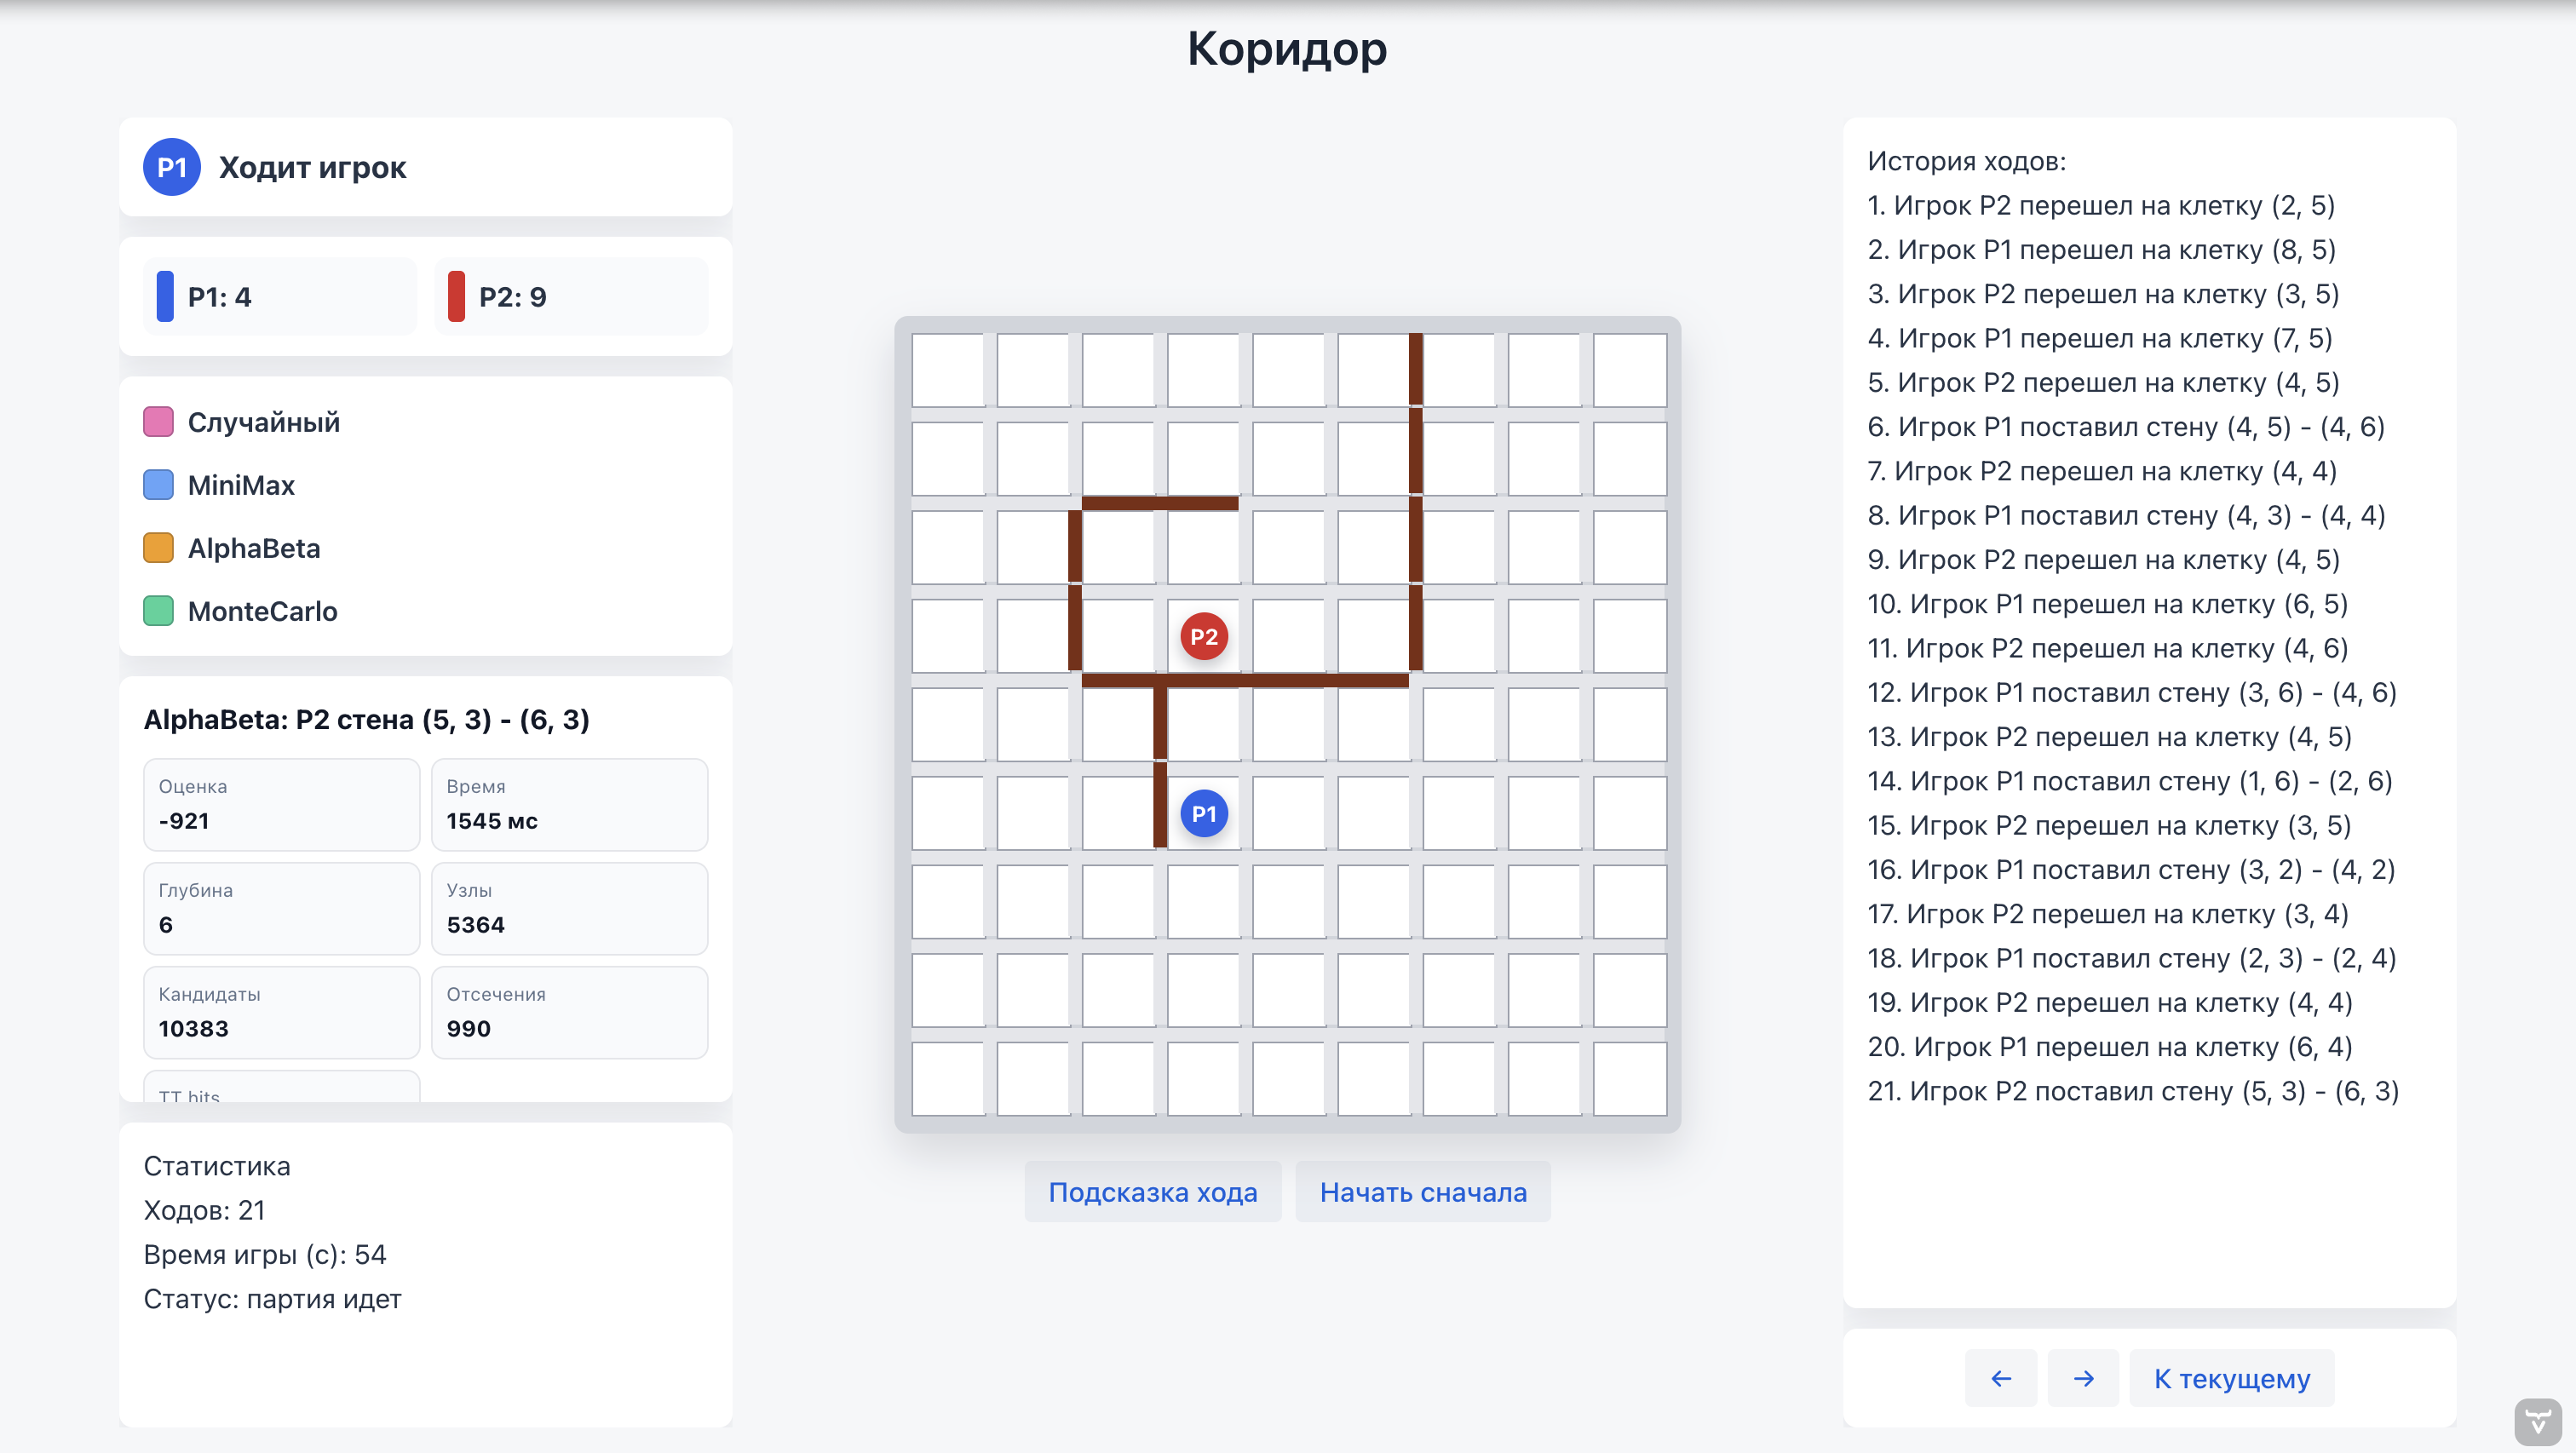
\includegraphics[width=0.88\textwidth]{game-page.png}
    \caption{Пример партии в приложении <<Коридор>>}
    \label{fig:intro_game}
\end{figure}

Игра получила заметное распространение среди настольных логических игр; в частности, она входила в подборку Games 100 журнала \textit{Games} \cite{games100}. Для данной работы важен не только прикладной интерфейс игры, но и математическая структура задачи: <<Коридор>> удобно рассматривать как задачу принятия решений на графе. Клетки поля соответствуют вершинам графа $G = (V, E)$, допустимые переходы между соседними клетками "--- рёбрам. Установленная перегородка удаляет из $E$ одно или несколько рёбер. Ключевое ограничение правил — перегородка не может полностью перекрыть путь ни одного из игроков к его целевой линии — требует после каждого потенциального изменения структуры графа проверять наличие хотя бы одного маршрута у обоих участников.

Задача разработки программного соперника для подобных игр является классической в области игрового искусственного интеллекта. Для игр с полной информацией и нулевой суммой, к которым относится <<Коридор>>, традиционно применяются алгоритмы на основе дерева игровых состояний: минимакс и его расширения \cite{Russell:2021}. Альтернативным подходом является метод Монте-Карло (MCTS) \cite{Coulom:2006}, не требующий явной оценочной функции.

Целью выпускной квалификационной работы является разработка игрового приложения <<Коридор>>, включающего реализацию правил игры, визуализацию игрового поля и модуль стратегического поведения, объединяющий четыре алгоритма программного соперника. Проведённое сравнение алгоритмов в серии автоматических партий позволяет оценить их относительную силу.

Для реализации цели работы были поставлены следующие задачи:

\begin{enumerate}
    \item изучить правила игры <<Коридор>> и построить графовую модель игрового поля,
    \item реализовать алгоритм проверки корректности перемещения фишки, включая прыжки через соперника,
    \item реализовать алгоритм проверки корректности установки перегородки с проверкой достижимости целевых линий,
    \item реализовать алгоритм поиска кратчайшего пути до целевой линии на основе обхода графа в ширину,
    \item разработать многофакторную функцию оценки игровой позиции с настраиваемыми весами и механизмом их онлайн-коррекции по результатам партий,
    \item реализовать четыре алгоритма программного соперника: случайный выбор, минимакс, минимакс с альфа-бета отсечением и MCTS,
    \item провести сравнение алгоритмов в серии автоматических партий,
    \item разработать интерфейс игрового приложения с поддержкой режимов <<Игрок против ИИ>>, <<ИИ против ИИ>>, режима подсказок и воспроизведения партии.
\end{enumerate}

\chapter{Игра <<Коридор>>}

\section{Необходимые определения}

В формулировке правил игры и последующем описании алгоритмов встречается несколько понятий, которые нуждаются в пояснении.

\textit{Игровым полем} называется квадратная доска размером $n \times n$ клеток, по которым перемещаются фишки игроков. В стандартном варианте $n = 9$; приложение также поддерживает поля $7 \times 7$ и $11 \times 11$. Клетки нумеруются парами $(i, j)$, где $0 \le i, j \le n - 1$.

\textit{Фишкой} называется объект, расположенный ровно в одной клетке поля. В двухпользовательском варианте игры участвуют две фишки.

\textit{Перегородкой} называется элемент, размещаемый на границе между клетками. Перегородка занимает два смежных межклеточных промежутка и может быть ориентирована горизонтально (блокирует переходы вверх–вниз между двумя парами клеток) или вертикально (блокирует переходы влево–вправо). Каждый игрок располагает фиксированным числом перегородок, зависящим от размера поля: 8 для поля $7 \times 7$, 10 для $9 \times 9$, 12 для $11 \times 11$.

\textit{Целевой линией} игрока называется строка, противоположная от его стартовой позиции. Первый игрок стартует из центра последней строки и стремится к строке $i = 0$; второй "--- из центра первой строки и стремится к строке $i = n - 1$.

\textit{Состоянием игры} называется кортеж $(p_1, p_2, W, w_1, w_2, t)$, где $p_1, p_2$ "--- позиции фишек; $W$ "--- множество установленных перегородок; $w_1, w_2$ "--- количества оставшихся перегородок у каждого игрока; $t \in \{1, 2\}$ "--- номер игрока, совершающего текущий ход.

\textit{Графовой моделью} игрового поля является неориентированный граф $G = (V, E)$, где $V$ "--- множество клеток ($|V| = n^2$), а $E$ "--- множество допустимых переходов между соседними клетками. Установка перегородки удаляет из $E$ два ребра. В приложении граф хранится в виде хеш-таблицы: каждой клетке $(i, j)$ сопоставлен объект \texttt{BoardTile} с четырьмя булевыми полями "--- флагами доступности переходов в четырёх направлениях: влево, вперёд (убывание $i$), вправо и назад (возрастание $i$).

\section{Описание игры}

Игра <<Коридор>> была выпущена компанией Gigamic в 1997 году. Впоследствии она была переведена на несколько языков и распространилась по всему миру, став предметом изучения в области игрового искусственного интеллекта.

В начале партии фишки расставляются на противоположных сторонах поля: первый игрок "--- в центре нижней строки, второй "--- в центре верхней строки. Игроки ходят по очереди, начиная с того, кому выпал жребий. Цель каждого игрока "--- первым достичь любой клетки своей целевой линии.

За один ход игрок выполняет ровно одно из двух действий.

\textit{Перемещение фишки.} Фишка перемещается на соседнюю клетку по горизонтали или вертикали при условии, что между ними нет перегородки. Если соседняя клетка занята фишкой соперника и за ней нет перегородки и нет границы поля, разрешается прыжок через соперника (фишка перемещается через него). Если прямой прыжок невозможен из-за перегородки или края поля, допускается диагональный ход: фишка перемещается на клетку, расположенную под углом 90° относительно направления прыжка, при условии отсутствия перегородки в этом направлении.

\textit{Установка перегородки.} Игрок выбирает позицию и ориентацию перегородки. Установка допускается, если: у игрока есть хотя бы одна неиспользованная перегородка; новая перегородка не пересекается и не совпадает с уже установленными; после её установки у каждого игрока сохраняется хотя бы один маршрут к своей целевой линии.

Партия завершается, когда фишка одного из игроков достигает любой клетки целевой линии. Этот игрок объявляется победителем.

\section{Модуль стратегического поведения}

Модуль стратегического поведения представляет собой программный компонент, отвечающий за выбор хода программным соперником. Он получает на вход текущее состояние игры, количество оставшихся перегородок у каждого из игроков и возвращает выбранный ход.

Требования к модулю формулируются следующим образом.

\begin{enumerate}
    \item \textit{Корректность}: выбираемый ход всегда должен быть допустимым с точки зрения правил игры. В приложении реализован дополнительный уровень защиты: если алгоритм по какой-либо причине возвращает недопустимый ход, \texttt{GameProcessor} автоматически подменяет его наилучшим доступным ходом фишкой, выбранным по эвристике близости к целевой линии и штрафа за повторение позиций.
    \item \textit{Завершённость}: алгоритм должен завершаться за конечное время. Все переборные алгоритмы (минимакс, альфа-бета, MCTS) работают с ограничением по времени: каждый из них получает лимит в миллисекундах и прекращает поиск по его истечении.
    \item \textit{Единый интерфейс}: все стратегии реализуют интерфейс \texttt{Algorithm} с методом \texttt{getMove(board, hardnessLevel, playerId, wallsLeft1, wallsLeft2)}. Это позволяет переключать алгоритмы без изменения остальных компонентов приложения.
    \item \textit{Настраиваемая сложность}: каждый алгоритм поддерживает три уровня сложности "--- \texttt{EASY}, \texttt{MEDIUM} и \texttt{HARD}, которые влияют на глубину поиска, лимит времени и число итераций.
    \item \textit{Масштабируемость}: архитектура допускает добавление новых алгоритмов без изменения существующих компонентов через \texttt{ComputerPlayerFabric}.
\end{enumerate}

В рамках данной работы в модуле реализованы четыре стратегии. Случайный алгоритм (\texttt{RandomAlgorithm}) равновероятно выбирает ход из множества допустимых и служит базовой линией для сравнения. Минимакс (\texttt{MinimaxAlgorithm}) перебирает дерево игровых состояний на ограниченную глубину без каких-либо отсечений. Альфа-бета (\texttt{AlphaBetaAlgorithm}) реализует минимакс с отсечениями, сортировкой ходов и таблицей транспозиций. Метод Монте-Карло (\texttt{MonteCarloAlgorithm}) оценивает позиции через многократные случайные симуляции с использованием формулы UCT.

\chapter{Алгоритмы}

\section{Общие функции и структура алгоритмов}

Все четыре алгоритма программного соперника реализуют интерфейс \texttt{Algorithm}, содержащий как абстрактные методы, так и конкретные реализации вспомогательных функций по умолчанию (\texttt{default}-методы Java). Такой подход исключает дублирование кода и гарантирует единообразное поведение алгоритмов в одинаковых ситуациях.

\subsection*{Генерация допустимых ходов}

Метод \texttt{getMoves(board, playerId, wallsLeft)} формирует полное множество допустимых ходов из текущего состояния. Оно складывается из двух частей.

Первая часть "--- допустимые перемещения фишки. Они получаются вызовом \texttt{board.getAvailableMoves(pos)}, который обходит четыре направления от текущей позиции, проверяя флаги \texttt{BoardTile}, и обрабатывает прыжки через соперника: прямой прыжок добавляется, если за фишкой соперника нет перегородки и нет края поля; в противном случае добавляются диагональные прыжки в обе стороны при их доступности.

Вторая часть "--- допустимые установки перегородок. Если у игрока не осталось перегородок (\texttt{wallsLeft <= 0}), эта часть пуста. В противном случае алгоритм формирует множество \textit{кандидатных клеток}, ограничивая полный перебор стратегически значимой областью поля. Кандидатами являются: первые 12 клеток кратчайшего пути соперника к его целевой линии; первые 7 клеток кратчайшего пути самого алгоритма; окрестность радиуса 2 вокруг фишки соперника; окрестность радиуса 1 вокруг первых 5 клеток пути соперника. Для каждой кандидатной клетки проверяются два возможных направления перегородки "--- вертикальное и горизонтальное. Перегородка включается в список кандидатов, если она физически размещаема (\texttt{isWallPlaceable}) и не отрезает ни одного из игроков от его целевой линии (\texttt{isValidWall}), причём выполняется хотя бы одно из условий стратегической ценности: перегородка удлиняет путь соперника не менее чем на 2 хода; соперник находится в 3 ходах от победы и перегородка его замедляет; перегородка удлиняет путь соперника не меньше, чем собственный путь алгоритма. Финальный список перегородок сортируется по убыванию функции \texttt{wallImpact}.

\subsection*{Поиск кратчайшего пути}

Метод \texttt{calculateShortestPath(board, start, targetRow)} реализует обход графа в ширину (BFS) от стартовой позиции до ближайшей клетки целевой строки. Алгоритм использует очередь уровней: на каждой итерации внешнего цикла обрабатывается весь текущий уровень, после чего счётчик глубины увеличивается на 1. Возвращается длина кратчайшего пути в ходах; если путь не найден "--- возвращается значение 1000 (условная бесконечность). Трудоёмкость одного вызова составляет $O(|V| + |E|)$, что при фиксированном размере поля эквивалентно $O(1)$ по параметрам задачи.

Метод \texttt{getShortestPathCells} дополняет BFS восстановлением пути через хранение родителей и используется при генерации кандидатных клеток для установки перегородок.

\subsection*{Эндшпильные правила}

Метод \texttt{findEndgameMove} применяется всеми четырьмя алгоритмами как первый шаг перед запуском основного поиска. Если из текущей позиции фишку можно переместить прямо на целевую линию "--- этот ход немедленно возвращается без какого-либо перебора. Если такого хода нет, но соперник находится не далее чем в двух ходах от победы и у алгоритма есть перегородки "--- ищется перегородка с максимальным значением \texttt{wallImpact}, замедляющая соперника.

\subsection*{Предпочтение направления движения}

Метод \texttt{movementPreference} добавляет к оценке хода бонус или штраф в зависимости от направления и истории позиций:

\begin{itemize}
    \item ход вперёд (в сторону целевой линии): $+45$ очков;
    \item ход назад: $-120$ очков;
    \item приближение к целевой линии на $\Delta$ клеток: $+35 \cdot \Delta$ очков;
    \item повторение позиции, встречавшейся 1--2 хода назад: $-500$ очков;
    \item повторение более давней позиции: $-180$ очков.
\end{itemize}

История позиций хранится для каждого игрока отдельно в \texttt{GameProcessor} и передаётся в алгоритм через метод \texttt{setRecentPositions}.

\subsection*{Функция оценки позиции}

Функция оценки \texttt{evaluate(board, playerId, size, wallsLeft1, wallsLeft2)} является центральным компонентом всех переборных алгоритмов. Она ставит в соответствие каждому нетерминальному состоянию игры числовое значение, характеризующее его выгодность для программного соперника. Если состояние терминальное "--- победа алгоритма или пользователя "--- функция возвращает $+\mathrm{WIN\_SCORE} + d$ или $-\mathrm{WIN\_SCORE} - d$ соответственно, где $\mathrm{WIN\_SCORE} = 100\,000$, а $d$ "--- текущая глубина поиска (это обеспечивает предпочтение более близкой победы).

Для нетерминальных состояний оценка вычисляется как взвешенная сумма семи признаков:

\begin{equation}
    F(s) = \sum_{k=1}^{7} \lambda_k \cdot f_k(s),
\end{equation}

где $\lambda_k$ "--- веса, а $f_k(s)$ "--- значения признаков. Признаки и их смысл перечислены в таблице~\ref{tab:features}.

\begin{table}[h]
    \centering
    \caption{Признаки оценочной функции}
    \label{tab:features}
    \begin{tabular}{clp{7cm}}
        \toprule
        $k$ & Признак $f_k(s)$ & Описание \\
        \midrule
        1 & $d_p - d_a$ & Разность длин кратчайших путей: путь пользователя минус путь алгоритма \\
        2 & $\mathrm{mob}_a$ & Количество допустимых ходов фишкой алгоритма \\
        3 & $-\mathrm{mob}_p$ & Отрицательное количество допустимых ходов пользователя \\
        4 & $w_a - w_p$ & Преимущество алгоритма по числу оставшихся перегородок \\
        5 & $\mathrm{prog}_a - \mathrm{prog}_p$ & Разность продвижений к целевым линиям \\
        6 & $e(d_a)$ & Эндшпильный бонус за близость алгоритма к победе \\
        7 & $-e(d_p)$ & Эндшпильный штраф за близость пользователя к победе \\
        \bottomrule
    \end{tabular}
\end{table}

Продвижение $\mathrm{prog}_a$ вычисляется как количество строк, пройденных фишкой алгоритма от стартовой позиции до текущей. Эндшпильная функция $e(d)$ принимает значения:

\[
e(d) = \begin{cases}
    10, & d \le 1, \\
    4,  & d = 2, \\
    1,  & d = 3, \\
    0,  & d > 3.
\end{cases}
\]

Веса $\lambda_k$ по умолчанию заданы следующим образом (класс \texttt{EvaluationWeights}):

\[
\lambda_1 = 65,\quad \lambda_2 = 4,\quad \lambda_3 = 3,\quad \lambda_4 = 18,\quad \lambda_5 = 6,\quad \lambda_6 = 165,\quad \lambda_7 = 175.
\]

\subsection*{Онлайн-коррекция весов}

Приложение реализует механизм автоматической коррекции весов функции оценки по результатам сыгранных партий (класс \texttt{EvaluationWeightsStore}). После завершения каждой партии, в которой участвовал программный соперник, вычисляется градиентная оценка полезности ходов.

В течение партии для каждого хода алгоритма формируется объект \texttt{EvaluationLearningSample}, хранящий вектор признаков до хода и после него (\texttt{EvaluationFeatures before, after}). После завершения партии для каждого образца вычисляется дельта признаков $\Delta f_k = f_k^{\mathrm{after}} - f_k^{\mathrm{before}}$ и суммируется в градиент с учётом знака:

\begin{equation}
    g_k = \sum_{\text{ходы алгоритма}} \mathrm{reward} \cdot \Delta f_k, \quad \mathrm{reward} = \begin{cases} +1, & \text{алгоритм победил}, \\ -1, & \text{алгоритм проиграл.} \end{cases}
\end{equation}

Веса обновляются по правилу:

\begin{equation}
    \lambda_k \leftarrow \mathrm{clamp}\bigl(\lambda_k + \mathrm{sign}(g_k) \cdot \Delta\lambda,\; \lambda_k^{\min},\; \lambda_k^{\max}\bigr),
\end{equation}

где $\Delta\lambda = 1$ "--- шаг обучения, $[\lambda_k^{\min}, \lambda_k^{\max}]$ "--- допустимый диапазон каждого веса, предотвращающий вырождение оценки. Актуальные веса сохраняются в файл \texttt{data/evaluation-weights.properties} и загружаются при следующем запуске приложения, что обеспечивает накопление опыта между сессиями. На момент написания работы механизм принял $15$ обновлений весов на $1388$ обучающих образцах, а текущие сохранённые веса составляют:

\[
\lambda_1 = 120,\quad \lambda_2 = 7,\quad \lambda_3 = 12,\quad \lambda_4 = 8,\quad \lambda_5 = 25,\quad \lambda_6 = 186,\quad \lambda_7 = 170.
\]

Сравнение начальных и сохранённых весов показывает, что механизм увеличил приоритет разности путей ($\lambda_1: 65 \to 120$), штрафа за мобильность соперника ($\lambda_3: 3 \to 12$), продвижения к цели ($\lambda_5: 6 \to 25$) и собственного эндшпильного преимущества ($\lambda_6: 165 \to 186$), одновременно снизив вес преимущества по оставшимся перегородкам ($\lambda_4: 18 \to 8$).

\subsection*{Функция wallImpact}

Функция \texttt{wallImpact(board, move, playerId, size)} оценивает стратегическую ценность конкретной установки перегородки. Она применяет ход к копии доски и вычисляет изменения длин путей:

\begin{equation}
    \mathrm{wallImpact} = (d_p^{\mathrm{after}} - d_p^{\mathrm{before}}) \cdot 100 - \max(0,\, d_a^{\mathrm{after}} - d_a^{\mathrm{before}}) \cdot 45,
\end{equation}

то есть каждый шаг, добавленный к пути соперника, оценивается в 100 единиц, а каждый шаг, добавленный к собственному пути, штрафуется 45 единицами. Перегородка считается стратегически ценной при \texttt{wallImpact} $> 0$.

\section{Случайный алгоритм}

Случайный алгоритм (\texttt{RandomAlgorithm}) является простейшим программным соперником и используется как базовая линия для сравнения. При каждом вызове метода \texttt{getMove} алгоритм первым делом применяет эндшпильное правило: если можно немедленно выиграть или срочно заблокировать соперника, он делает это независимо от уровня сложности. Если эндшпильное правило не сработало, поведение определяется уровнем сложности.

На уровне \texttt{EASY} алгоритм равновероятно выбирает ход из полного множества $M(s)$ допустимых ходов.

На уровне \texttt{MEDIUM} ходы сортируются по убыванию значения \texttt{evaluateAfterMove} (оценка позиции после совершения хода), и случайно выбирается один из первой половины списка.

На уровне \texttt{HARD} случайно выбирается один из трёх лучших ходов по той же оценке.

\begin{algorithm}
\caption{Случайный алгоритм}\label{alg:random}
эндшпильный ход $\leftarrow$ \texttt{findEndgameMove}$(s)$\;
\If{эндшпильный ход найден}{
    \KwRet{эндшпильный ход}
}
$M \leftarrow$ \texttt{getMoves}$(s)$\;
\uIf{уровень = \texttt{EASY}}{
    $m^* \leftarrow$ случайный элемент $M$\;
}
\uElseIf{уровень = \texttt{MEDIUM}}{
    сортировать $M$ по убыванию \texttt{evaluateAfterMove}\;
    $m^* \leftarrow$ случайный элемент из первой половины $M$\;
}
\Else{
    сортировать $M$ по убыванию \texttt{evaluateAfterMove}\;
    $m^* \leftarrow$ случайный элемент из первых трёх элементов $M$\;
}
\KwRet{$m^*$}
\end{algorithm}

Трудоёмкость алгоритма на уровне \texttt{EASY} определяется только генерацией ходов. Оценка каждого хода требует одного вызова BFS, поэтому на уровнях \texttt{MEDIUM} и \texttt{HARD} трудоёмкость составляет $O(|M(s)| \cdot |V|)$.

\section{Алгоритм минимакса}

Алгоритм минимакса (\texttt{MinimaxAlgorithm}) основан на предположении об оптимальной игре обоих участников \cite{Russell:2021}. На ходах программного соперника выбирается ход с максимальной оценкой (максимизирующий узел); на ходах пользователя предполагается выбор хода с минимальной оценкой (минимизирующий узел).

Алгоритм использует итеративное углубление: последовательно запускает поиск с глубиной $d = 1, 2, \ldots, d_{\max}$ до истечения лимита времени. Результат последнего завершённого поиска возвращается как ответ. Это обеспечивает всегда иметь допустимый ответ, даже если время закончилось прежде, чем поиск на очередной глубине был завершён.

Максимальная глубина $d_{\max}$ и лимит времени $T$ зависят от уровня сложности и размера поля:

\begin{table}[h]
    \centering
    \caption{Параметры минимакса}
    \label{tab:minimax_params}
    \begin{tabular}{lcc}
        \toprule
        Уровень & $d_{\max}$ (поле $9\times9$) & $T$, мс (поле $9\times9$) \\
        \midrule
        \texttt{EASY}   & 3 & 700  \\
        \texttt{MEDIUM} & 4 & 1800 \\
        \texttt{HARD}   & 5 & 3600 \\
        \bottomrule
    \end{tabular}
\end{table}

В целях ограничения времени работы ширина перебора ограничена функцией \texttt{limitMoves}: если число допустимых ходов превышает 16, список обрезается до первых 16 (порядок определяется генератором ходов). Для мемоизации использует таблица \texttt{cache}: ключ включает строковое представление доски, глубину, флаг максимизации и количества перегородок.

% \begin{algorithm}
% \caption{Минимакс}\label{alg:minimax}
% \SetKwFunction{FMM}{minimax}
% \SetKwProg{Fn}{Функция}{:}{}
% \Fn{\FMM{$s$, $d$, isMax}}
%     \If{в кэше есть результат для $(s, d, \mathrm{isMax})$}{
%         \KwRet{значение из кэша}
%     }
%     \If{$\mathrm{terminal}(s)$ \textbf{или} $d = 0$}{
%         \KwRet{$F(s)$}
%     }
%     $\mathrm{cur} \leftarrow$ игрок данного узла\;
%     $M \leftarrow$ \texttt{limitMoves}(\texttt{getMoves}$(s, \mathrm{cur})$)\;
%     $\mathrm{best} \leftarrow -\infty$ если isMax, иначе $+\infty$\;
%     \ForEach{$m \in M$}{
%         $s' \leftarrow \mathrm{apply}(s, m)$\;
%         $v \leftarrow$ \FMM{$s'$, $d-1$, $\neg$isMax}\;
%         $\mathrm{best} \leftarrow \max(\mathrm{best}, v)$ если isMax, иначе $\min(\mathrm{best}, v)$\;
%     }
%     сохранить $\mathrm{best}$ в кэше для $(s, d, \mathrm{isMax})$\;
%     \KwRet{$\mathrm{best}$
% }
% \BlankLine
% \ForEach{глубина $d = 1, 2, \ldots, d_{\max}$, пока не истёк лимит $T$}{
%     $m^* \leftarrow \arg\max_{m \in M(s)}$ \FMM{$\mathrm{apply}(s,m)$, $d-1$, \textbf{false}}\;
%     + \texttt{movementPreference}$(m, s)$\;
% }
% \KwRet{$m^*$}
% \end{algorithm}

Трудоёмкость в наихудшем случае "--- $O(b^d)$, где $b \le 16$ "--- ограниченная ширина перебора. При $d = 5$ это не более $16^5 \approx 1{,}05 \cdot 10^6$ узлов, что укладывается в лимит 3600 мс.

\section{Минимакс с альфа-бета отсечением}

Алгоритм альфа-бета (\texttt{AlphaBetaAlgorithm}) является наиболее сложным из реализованных. Он расширяет минимакс тремя независимыми механизмами ускорения: отсечениями, сортировкой ходов и таблицей транспозиций.

\subsection*{Альфа-бета отсечение}

Алгоритм поддерживает два параметра: $\alpha$ "--- наилучшая оценка, гарантированная максимизирующему игроку, и $\beta$ "--- наилучшая оценка, гарантированная минимизирующему. Если в ходе перебора $\beta \le \alpha$, оставшиеся ходы в данном узле можно не рассматривать: они не изменят итогового выбора. Это позволяет в лучшем случае сократить число рассматриваемых состояний до $O(b^{d/2})$.

\subsection*{Сортировка ходов}

Эффективность отсечений критически зависит от порядка рассмотрения ходов: если лучший ход рассматривается первым, отсечения происходят как можно раньше. Функция \texttt{scoreMove} оценивает каждый ход до его применения по нескольким критериям:
\begin{itemize}
    \item $+20\,000$, если ход совпадает с записью из таблицы транспозиций (\textit{лучший ход} из предыдущего поиска);
    \item $+10\,000$ / $+8\,000$, если ход является первым или вторым \textit{killer-ходом} данного уровня глубины;
    \item вес из таблицы \texttt{goodMoves} "--- истории ходов, вызывавших отсечения в предыдущих узлах;
    \item значение функции оценки после применения хода.
\end{itemize}

После сортировки список ходов обрезается до 36 кандидатов.

\subsection*{Таблица транспозиций}

Таблица транспозиций (\texttt{transpositionTable}) хранит результаты уже вычисленных позиций. Ключ "--- строковое представление доски, флаг текущего игрока и количества перегородок. Каждая запись содержит оценку, глубину поиска, тип границы (точная оценка \texttt{EXACT}, нижняя граница \texttt{LOWER} или верхняя граница \texttt{UPPER}) и лучший ход для данной позиции. При попадании в таблицу алгоритм:
\begin{itemize}
    \item если глубина записи $\ge$ текущей и тип \texttt{EXACT} "--- немедленно возвращает сохранённое значение;
    \item если тип \texttt{LOWER} "--- использует запись для ужесточения нижней границы $\alpha$;
    \item если тип \texttt{UPPER} "--- для ужесточения верхней границы $\beta$.
\end{itemize}

\subsection*{Затухающий поиск (Quiescence Search)}

В позициях, где один из игроков находится не далее 2 ходов от победы (\textit{шумные позиции}, \texttt{isNoisyPosition}), применяется расширенный поиск \texttt{quiescence}. Вместо немедленного возврата статической оценки алгоритм дополнительно рассматривает финальные ходы (перемещение фишки на целевую линию) и до 8 наиболее ценных установок перегородок с глубиной расширения 2. Это предотвращает ошибки горизонта "--- ситуации, когда статическая оценка не отражает угрозы, возникающей сразу после горизонта поиска.

Параметры алгоритма в зависимости от уровня сложности для поля $9\times9$:

\begin{table}[h]
    \centering
    \caption{Параметры альфа-бета алгоритма}
    \label{tab:ab_params}
    \begin{tabular}{lcc}
        \toprule
        Уровень & $d_{\max}$ & $T$, мс \\
        \midrule
        \texttt{EASY}   & 4 & 1300 \\
        \texttt{MEDIUM} & 6 & 3600 \\
        \texttt{HARD}   & 8 & 7600 \\
        \bottomrule
    \end{tabular}
\end{table}

\begin{algorithm}
\caption{Альфа-бета с таблицей транспозиций}\label{alg:alphabeta}
\SetKwFunction{FAB}{alphabeta}
\SetKwProg{Fn}{Функция}{:}{}
\Fn{\FAB{$s$, $d$, $\alpha$, $\beta$, isMax}}{
    \If{запись $(s, d) \in$ TT}{
        скорректировать $\alpha$, $\beta$ по типу записи\;
        \If{$\alpha \ge \beta$}{ \KwRet{оценку из TT} }
    }
    \If{$\mathrm{terminal}(s)$}{ \KwRet{терминальная оценка} }
    \If{$d = 0$}{
        \eIf{\texttt{isNoisyPosition}$(s)$}{
            \KwRet{\texttt{quiescence}$(s, \alpha, \beta, \mathrm{isMax}, 2)$}
        }{
            \KwRet{$F(s)$}
        }
    }
    $M \leftarrow$ первые 36 ходов из \texttt{getMoves}$(s)$, отсортированных по \texttt{scoreMove}\;
    $\mathrm{best} \leftarrow -\infty$ если isMax, иначе $+\infty$\;
    \ForEach{$m \in M$}{
        $v \leftarrow$ \FAB{$\mathrm{apply}(s, m)$, $d-1$, $\alpha$, $\beta$, $\neg$isMax}\;
        обновить $\mathrm{best}$, $\alpha$ или $\beta$\;
        \If{$\beta \le \alpha$}{
            обновить killer-ходы и \texttt{goodMoves}\;
            \textbf{break} \tcp*{отсечение}
        }
    }
    сохранить $(\mathrm{best}, d, \text{тип})$ в TT\;
    \KwRet{$\mathrm{best}$}
}
\end{algorithm}

\section{Метод Монте-Карло (MCTS)}

Алгоритм Монте-Карло (\texttt{MonteCarloAlgorithm}) строит статистику по многократным симуляциям от текущей позиции до конца партии \cite{Coulom:2006}. В отличие от минимакса и альфа-бета, он не перебирает дерево равномерно до фиксированной глубины, а постепенно концентрирует вычислительный бюджет на наиболее перспективных ветвях. В реализации дополнительно используется эвристическая оценка позиции: она входит в UCT как небольшой нормализованный член и применяется при выборе ходов во время rollout. Структура алгоритма "--- дерево узлов, каждый из которых соответствует некоторому состоянию игры и хранит счётчики посещений $n_v$ и побед $w_v$.

Основной цикл алгоритма состоит из четырёх фаз.

\textit{Выбор (Selection).} Начиная с корня, алгоритм спускается по дереву, на каждом шаге выбирая дочерний узел с максимальным значением UCT:

\begin{equation}
    \mathrm{UCT}(v) = \frac{w_v}{n_v} + C \cdot \sqrt{\frac{\ln n_{\mathrm{parent}}}{n_v}} + h(v),
\end{equation}

где $C = 1{,}2$ "--- константа исследования; $h(v)$ "--- нормализованная эвристическая оценка $0{,}15 \cdot \tanh(F(s_v) / 500)$, добавляющая информацию о позиции без полного доминирования над статистикой. Если узел ни разу не посещался, ему присваивается приоритет $+\infty$.

\textit{Расширение (Expansion).} Когда все допустимые ходы из узла уже рассматривались в дочерних узлах, выбранный узел помечается как полностью расширенный. Иначе из списка ещё не рассмотренных ходов (предварительно отсортированных по \texttt{scoreMove}) берётся первый, и создаётся новый дочерний узел.

\textit{Симуляция (Simulation).} Из нового узла проводится случайная игра до терминального состояния или до исчерпания лимита шагов \texttt{rolloutDepth}. На каждом ходу симуляции применяется эвристика epsilon-greedy:
\begin{enumerate}
    \item если есть ход, немедленно завершающий партию "--- он выбирается;
    \item если соперник находится не далее 2 ходов от победы и у текущего игрока есть перегородки "--- выбирается перегородка с максимальным \texttt{wallImpact} (если её \texttt{wallImpact} > 0);
    \item с вероятностью $0{,}22$ "--- случайный ход из полного списка;
    \item иначе "--- из случайной выборки 18 ходов выбирается один из четырёх лучших по \texttt{scoreRolloutMove}.
\end{enumerate}

\textit{Обратное распространение (Backpropagation).} Результат симуляции распространяется вверх: для каждого узла на пути от листа к корню инкрементируются $n_v$ и $w_v$ (если результат является победой корневого игрока).

После истечения лимита времени или достижения бюджета итераций выбирается ход с наибольшим значением $n_c + w_c / n_c$ среди дочерних узлов корня (\textit{robustChild}), что отдаёт предпочтение хорошо исследованным ходам.

Параметры алгоритма для поля $9\times9$:

\begin{table}[h]
    \centering
    \caption{Параметры MCTS}
    \label{tab:mcts_params}
    \begin{tabular}{lccc}
        \toprule
        Уровень & Бюджет итераций & $T$, мс & Глубина симуляции \\
        \midrule
        \texttt{EASY}   & 520  & 950  & $9 \cdot 4 = 36$ \\
        \texttt{MEDIUM} & 1700 & 2900 & $9 \cdot 7 = 63$ \\
        \texttt{HARD}   & 3400 & 6200 & $9 \cdot 10 = 90$ \\
        \bottomrule
    \end{tabular}
\end{table}

\begin{algorithm}
\caption{MCTS}\label{alg:mcts}
$r \leftarrow$ корневой узел с состоянием $s$\;
\While{не истёк лимит $T$ \textbf{и} итераций $< N$}{
    $v \leftarrow \mathrm{select}(r)$ \tcp*{спуск по UCT}
    \If{$\neg\,\mathrm{terminal}(v.s)$}{
        $v \leftarrow \mathrm{expand}(v)$ \tcp*{новый дочерний узел}
    }
    $\mathrm{result} \leftarrow \mathrm{simulate}(v, \mathrm{rolloutDepth})$\;
    $\mathrm{backpropagate}(v, \mathrm{result})$\;
    \If{$r.n > 300$ \textbf{и} $\max_c(w_c/n_c) > 0.97$}{\textbf{break}}
}
\KwRet{$\arg\max_{c \in \mathrm{children}(r)} (n_c + w_c / n_c)$}
\end{algorithm}

Условие досрочного выхода (\texttt{bestWinRate > 0.97} при более чем 300 посещениях корня) позволяет экономить время в позициях, где один из ходов явно доминирует по статистике.

\section{Сводные параметры сложности}

Для удобства настройки экспериментов все уровни сложности сведены в таблицу~\ref{tab:all_difficulty_params}. Значения приведены для стандартного поля $9\times9$, поскольку именно оно используется в базовом сравнении алгоритмов. Для полей $7\times7$ и $11\times11$ параметры масштабируются в коде: на малом поле AlphaBeta может увеличивать глубину поиска, а на большом поле MiniMax и AlphaBeta уменьшают глубину либо увеличивают временной лимит, чтобы партия оставалась интерактивной.

\begin{table}[h]
    \centering
    \caption{Параметры уровней сложности алгоритмов для поля $9\times9$}
    \label{tab:all_difficulty_params}
    \begin{tabular}{llp{8cm}}
        \toprule
        Алгоритм & Уровень & Параметры \\
        \midrule
        Random & \texttt{EASY} & Случайный выбор среди всех допустимых ходов \\
        Random & \texttt{MEDIUM} & Случайный выбор из верхней половины ходов по функции оценки \\
        Random & \texttt{HARD} & Случайный выбор из трёх лучших ходов по функции оценки \\
        MiniMax & \texttt{EASY} & Глубина 3, лимит 700 мс, ширина перебора до 16 ходов \\
        MiniMax & \texttt{MEDIUM} & Глубина 4, лимит 1800 мс, ширина перебора до 16 ходов \\
        MiniMax & \texttt{HARD} & Глубина 5, лимит 3600 мс, ширина перебора до 16 ходов \\
        AlphaBeta & \texttt{EASY} & Глубина 4, лимит 1300 мс, сортировка ходов, до 36 кандидатов \\
        AlphaBeta & \texttt{MEDIUM} & Глубина 6, лимит 3600 мс, таблица транспозиций, killer-ходы \\
        AlphaBeta & \texttt{HARD} & Глубина 8, лимит 7600 мс, quiescence search в шумных позициях \\
        MCTS & \texttt{EASY} & До 520 итераций, лимит 950 мс, глубина rollout $9\cdot4=36$ \\
        MCTS & \texttt{MEDIUM} & До 1700 итераций, лимит 2900 мс, глубина rollout $9\cdot7=63$ \\
        MCTS & \texttt{HARD} & До 3400 итераций, лимит 6200 мс, глубина rollout $9\cdot10=90$ \\
        \bottomrule
    \end{tabular}
\end{table}

\chapter{Игровое приложение}

\section{Техническая реализация}

Игровое приложение написано на языке программирования Java версии 17 с использованием фреймворка Spring Boot версии 3.2.5, а также библиотеки Vaadin версии 24.4.2 \cite{vaadin}, обеспечивающей отрисовку игрового поля и взаимодействие с пользователем через веб-интерфейс. Для сокращения шаблонного кода используется библиотека Lombok. Система сборки "--- Maven.

Архитектура приложения разделена на несколько независимых слоёв. Общая схема взаимодействия слоёв представлена на рисунке~\ref{fig:architecture}.

\begin{figure}[h]
    \centering
    \begin{tikzpicture}[
        node distance=0.75cm,
        layer/.style={
            rectangle,
            rounded corners,
            draw=black!55,
            fill=gray!8,
            text width=10.5cm,
            align=center,
            minimum height=1.05cm
        },
        arr/.style={-{Latex[length=3mm]}, thick}
    ]
        \node[layer] (ui) {\textbf{UI Vaadin}\\ \texttt{StartPageController}, \texttt{GamePageController}, \texttt{TournamentPageController}, \texttt{AlgorithmComparisonPageController}};
        \node[layer, below=of ui] (service) {\textbf{Сервисный слой}\\ \texttt{GameProcessor}, \texttt{GameRules}, \texttt{TournamentService}, \texttt{SelfPlayTrainingService}, \texttt{BoardAnalyzer}};
        \node[layer, below=of service] (ai) {\textbf{Модуль стратегического поведения}\\ \texttt{RandomAlgorithm}, \texttt{MinimaxAlgorithm}, \texttt{AlphaBetaAlgorithm}, \texttt{MonteCarloAlgorithm}};
        \node[layer, below=of ai] (model) {\textbf{Игровая модель}\\ \texttt{Game}, \texttt{Board}, \texttt{BoardTile}, \texttt{Move}, \texttt{Position}, \texttt{Player}};
        \node[layer, below=of model] (storage) {\textbf{Файлы данных}\\ \texttt{data/evaluation-weights.properties}, \texttt{data/evaluation-weights-history.csv}};
        \draw[arr] (ui) -- (service);
        \draw[arr] (service) -- (ai);
        \draw[arr] (service) -- (model);
        \draw[arr] (ai) -- (model);
        \draw[arr] (ai) -- (storage);
    \end{tikzpicture}
    \caption{Общая архитектура приложения}
    \label{fig:architecture}
\end{figure}

\textit{Модель} (\texttt{ru.ac.uniyar.model}) содержит классы, описывающие игровые объекты. Класс \texttt{Position} хранит координаты клетки $(i, j)$ и предоставляет метод \texttt{move(rowDelta, colDelta)} для вычисления соседней позиции. Класс \texttt{BoardTile} описывает одну клетку поля четырьмя булевыми флагами доступности переходов. Класс \texttt{Board} хранит граф поля в виде \texttt{HashMap<Position, BoardTile>}, позиции фишек обоих игроков и реализует все операции с доской: размещение перегородок (\texttt{placeWall}), получение доступных ходов (\texttt{getAvailableMoves}), обход для BFS (\texttt{getPathNeighbors}) и полное копирование (\texttt{copy}). Класс \texttt{Move} описывает ход: его тип (\texttt{MOVE\_PLAYER} или \texttt{PLACE\_WALL}), идентификатор игрока и позиции начала и конца. Класс \texttt{Game} хранит конфигурацию текущей партии: размер поля (\texttt{GameSize}), ссылки на игроков, номер текущего хода, время начала и флаг завершения.

\textit{Игроки} (\texttt{ru.ac.uniyar.model.players}) реализуют иерархию через абстрактный класс \texttt{Player} с методом \texttt{getMove}. Класс \texttt{HumanPlayer} возвращает \texttt{null} (ход запрашивается через UI); класс \texttt{ComputerPlayer} делегирует вызов конкретному объекту \texttt{Algorithm}. Фабрика \texttt{ComputerPlayerFabric} создаёт нужную реализацию алгоритма по типу и уровню сложности.

\textit{Алгоритмы} (\texttt{ru.ac.uniyar.model.algorithms}) описаны в главе 2. Все реализуют интерфейс \texttt{Algorithm}. Класс \texttt{AlgorithmReport} является неизменяемой записью с результатами последнего хода: выбранный ход, оценка, достигнутая глубина, число рассмотренных узлов, число отсечений, число попаданий в таблицу транспозиций, время в миллисекундах и текстовое пояснение. Класс \texttt{EvaluationFeatures} хранит вектор признаков состояния; \texttt{EvaluationWeights} "--- веса; \texttt{EvaluationWeightsStore} управляет загрузкой и сохранением весов.

\textit{Сервисный слой} (\texttt{ru.ac.uniyar.service}) включает три компонента. \texttt{BoardFactory} создаёт начальное состояние доски заданного размера. \texttt{GameRules} проверяет корректность установки перегородки через BFS и конвертирует координаты рендера в игровые координаты. \texttt{GameProcessor} "--- аннотированный \texttt{@SessionScope} Spring-компонент, управляющий всем жизненным циклом партии: запуск (\texttt{startNewGame}), выполнение ходов (\texttt{makeMove}, \texttt{makeComputerMove}), режим воспроизведения (\texttt{replayPrevious/Next/Live}), сбор образцов для обучения весов и получение подсказок от всех четырёх алгоритмов. \texttt{BoardAnalyzer} формирует текстовые пояснения к ходам ИИ. \texttt{TournamentService} реализует автоматические серии партий для турнира и сравнения алгоритмов.

\textit{Интерфейсный слой} (\texttt{ru.ac.uniyar.ui}) реализован через компоненты Vaadin. \texttt{StartPageController} отображает стартовый экран с выбором режима и параметров. \texttt{GamePageController} реализует основной экран игры: отрисовку доски в виде сетки \texttt{Div}-элементов, панель информации (\texttt{GameInfoPanel}), историю ходов (\texttt{GameHistoryPanel}), кнопки управления. \texttt{TournamentPageController} и \texttt{AlgorithmComparisonPageController} реализуют соответствующие режимы.

\section{Взаимодействие с приложением}

При запуске приложения пользователь попадает на стартовый экран, на котором настраиваются параметры предстоящей партии (рисунок~\ref{fig:start_page}).

\begin{figure}[h]
    \centering
    
\includegraphics[width=0.88\textwidth]{start-page.png}
    \caption{Стартовый экран выбора режима игры и алгоритмов}
    \label{fig:start_page}
\end{figure}

\textit{Выбор размера поля.} Доступны три варианта: малое поле $7 \times 7$ с 8 перегородками у каждого игрока, стандартное $9 \times 9$ с 10 перегородками, большое $11 \times 11$ с 12 перегородками. Размер поля влияет на все параметры алгоритмов: лимиты времени и максимальные глубины масштабируются пропорционально.

\textit{Выбор первого игрока.} Первым может управлять человек или один из четырёх алгоритмов ИИ. Если выбран ИИ, дополнительно настраивается его уровень сложности.

\textit{Выбор второго игрока.} Второй игрок всегда управляется ИИ; выбирается алгоритм и уровень сложности. Карточки профилей отображают краткое описание выбранной стратегии.

На игровом экране пользователь видит несколько областей. Пример этого экрана приведён выше на рисунке~\ref{fig:intro_game}.

\textit{Игровое поле} отрисовывается в виде сетки: клетки (тайлы) чередуются с промежутками (щелями), в которых размещаются перегородки. Каждая клетка имеет размер 42--50 пикселей в зависимости от размера поля. Фишки отображаются цветными кружками (синий "--- P1, красный "--- P2). Допустимые для перемещения клетки подсвечиваются зелёным при наведении. При наведении на щель между клетками предварительно подсвечивается потенциальная перегородка.

\textit{Перемещение фишки} выполняется кликом на целевую клетку. Если ход недопустим, появляется уведомление. Если ход совершается в режиме воспроизведения — он игнорируется.

\textit{Установка перегородки} выполняется кликом на промежуток между клетками. \texttt{GameRules.extractWall} определяет по координатам рендера начальную и конечную клетки перегородки. Затем \texttt{GameRules.canPlaceWall} копирует доску, применяет перегородку и проверяет достижимость целевых линий обоих игроков через BFS.

\textit{Ход ИИ.} В режиме <<Игрок против ИИ>> после хода пользователя автоматически запускается выбранный алгоритм. В режиме <<ИИ против ИИ>> каждый ход требует нажатия кнопки <<Сделать ход ИИ>>, что позволяет наблюдать за партией пошагово. Рядом с кнопкой отображается, чья очередь делать ход.

\textit{Подсказка.} Кнопка <<Подсказка хода>> запускает все четыре алгоритма на текущей позиции и подсвечивает рекомендованные ими ходы разными цветами: синий (MiniMax), жёлтый (AlphaBeta), зелёный (MonteCarlo), розовый (Random). Если несколько алгоритмов рекомендуют один ход "--- клетка закрашивается градиентом.

\textit{Панель информации} отображает: чья очередь; количество оставшихся перегородок у каждого игрока; легенду цветов алгоритмов; отчёт о последнем ходе ИИ (оценка, время, глубина, узлы, отсечения, попадания в TT, текстовое пояснение); статистику партии (число ходов, время).

\textit{Режим воспроизведения.} Кнопки «←», «→» и «К текущему» позволяют листать историю партии, просматривая состояние доски на любом из сыгранных ходов. История ходов дублируется текстовым списком в правой панели.

\textit{Турнирный режим} позволяет задать два алгоритма, их уровни сложности, размер поля и число партий. Результаты выводятся в режиме реального времени: по завершении каждой партии обновляется счётчик побед. По завершении серии выводится сводная таблица. Пример работы режима показан на рисунке~\ref{fig:tournament_page}.

\begin{figure}[h]
    \centering
    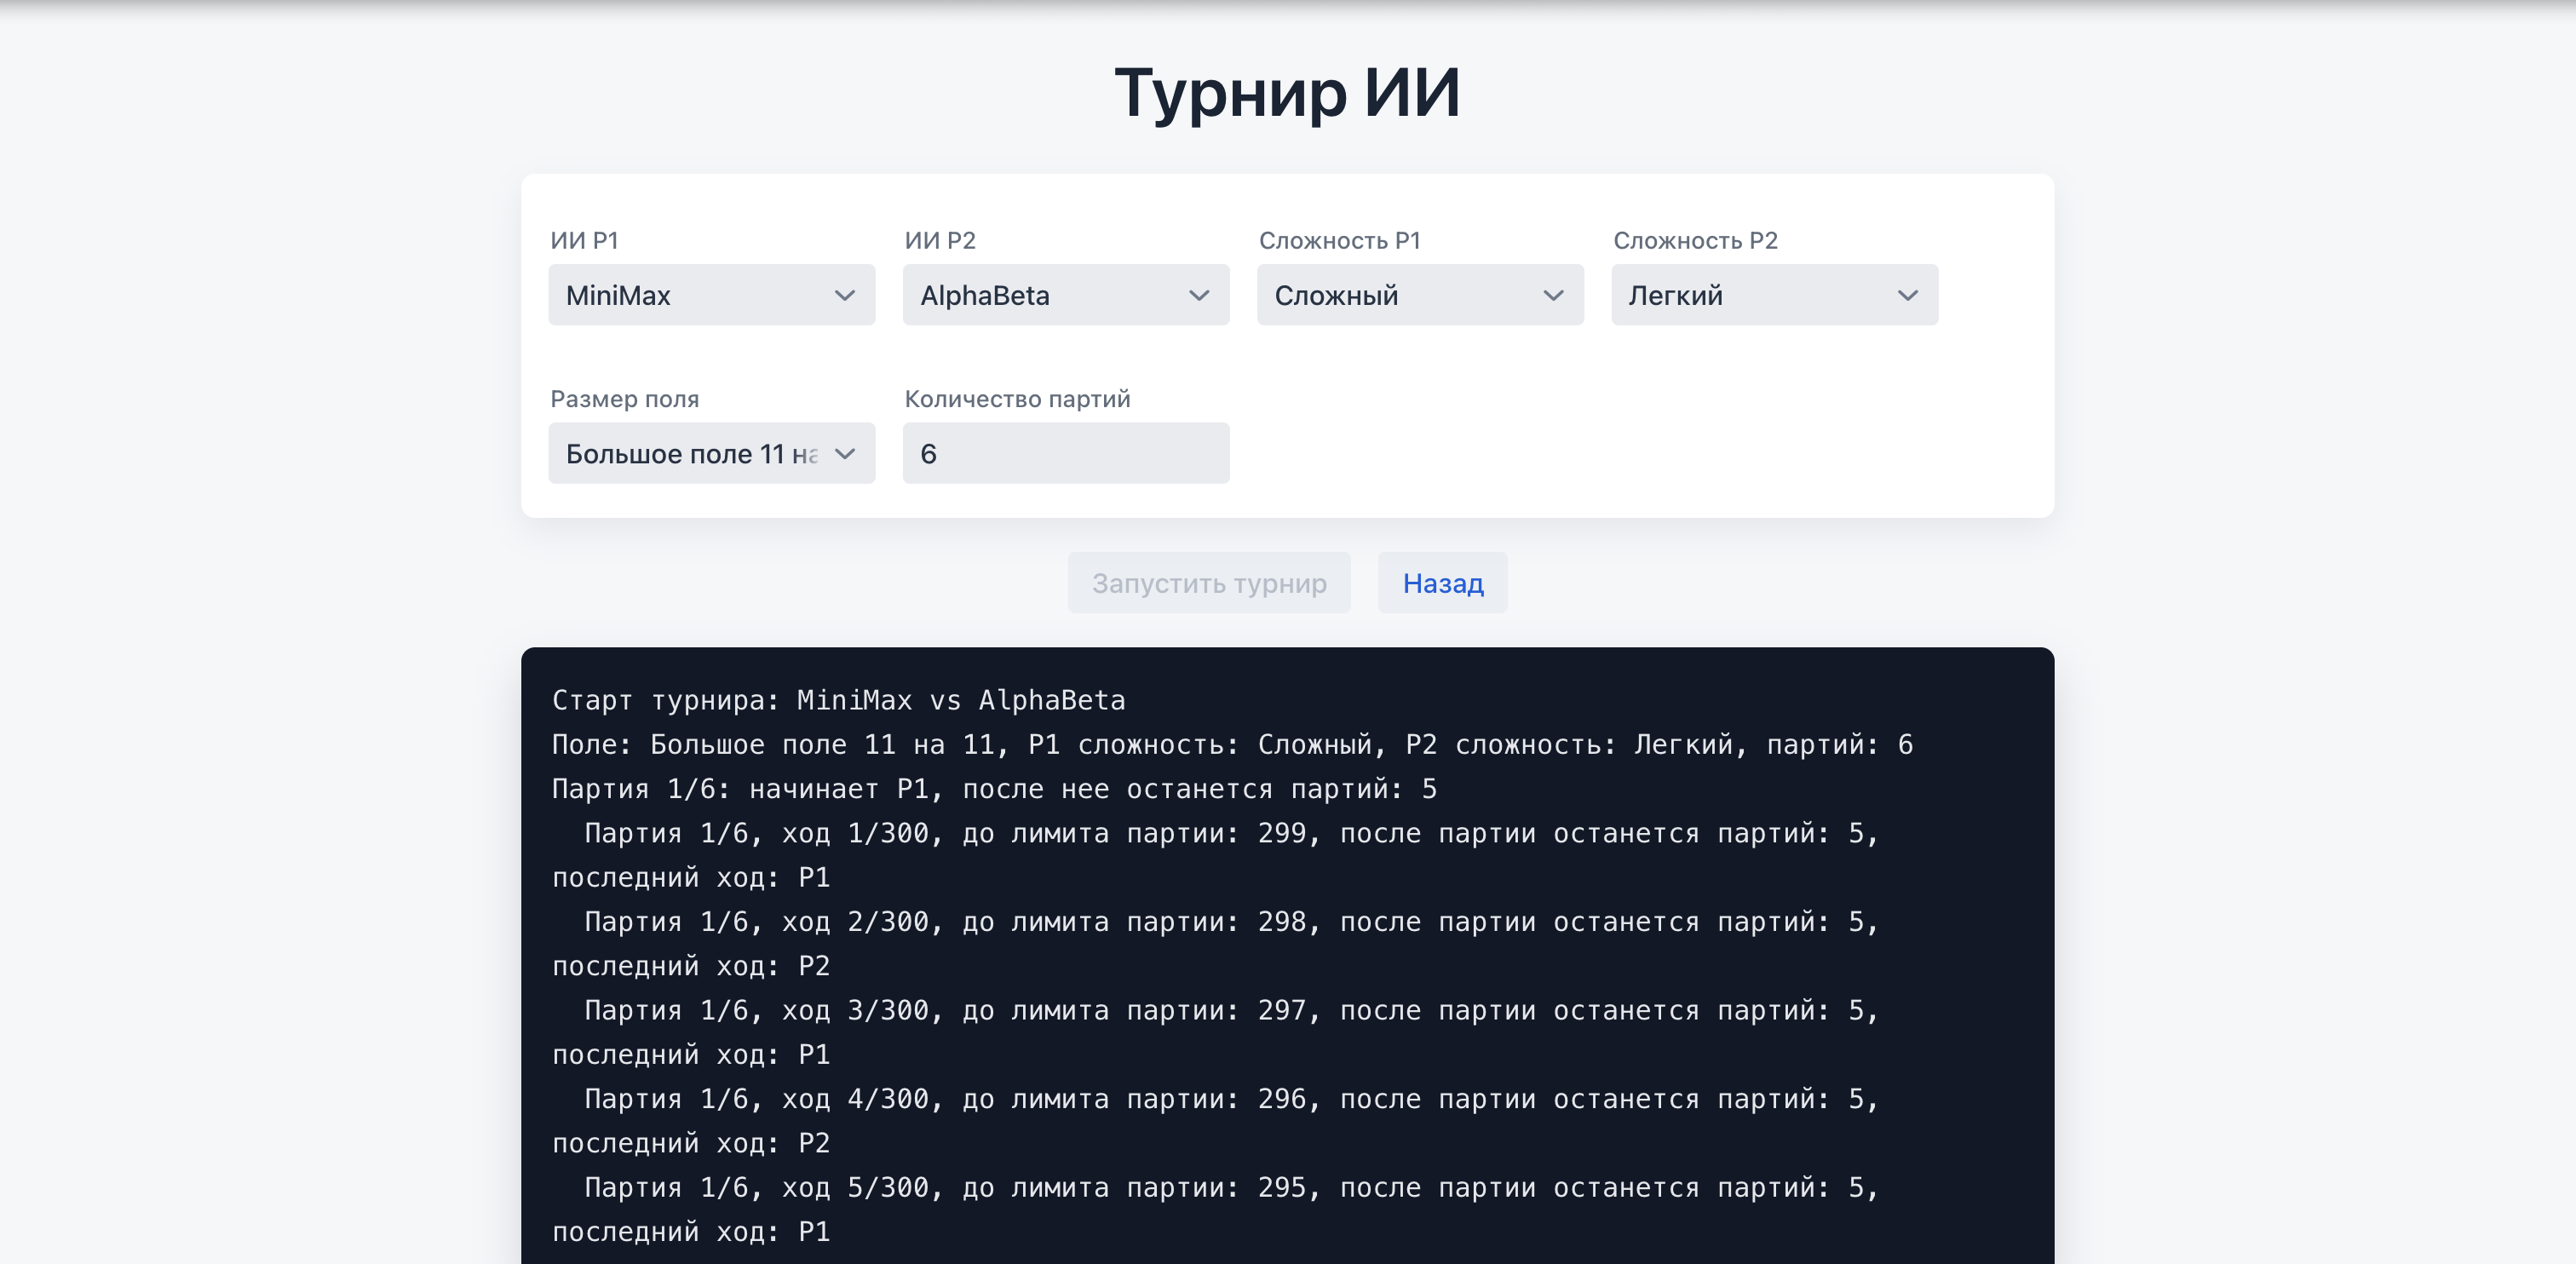
\includegraphics[width=0.88\textwidth]{tournament-page.png}
    \caption{Экран турнирного режима ИИ}
    \label{fig:tournament_page}
\end{figure}

\textit{Режим сравнения алгоритмов} автоматически проводит серию матчей между всеми попарными комбинациями четырёх алгоритмов (без зеркальных повторов) и выводит сводную таблицу с процентом побед, средним числом ходов, средним временем хода, средней глубиной поиска, числом узлов, отсечений и попаданий в TT. Интерфейс режима приведён на рисунке~\ref{fig:comparison_page}.

\begin{figure}[h]
    \centering
    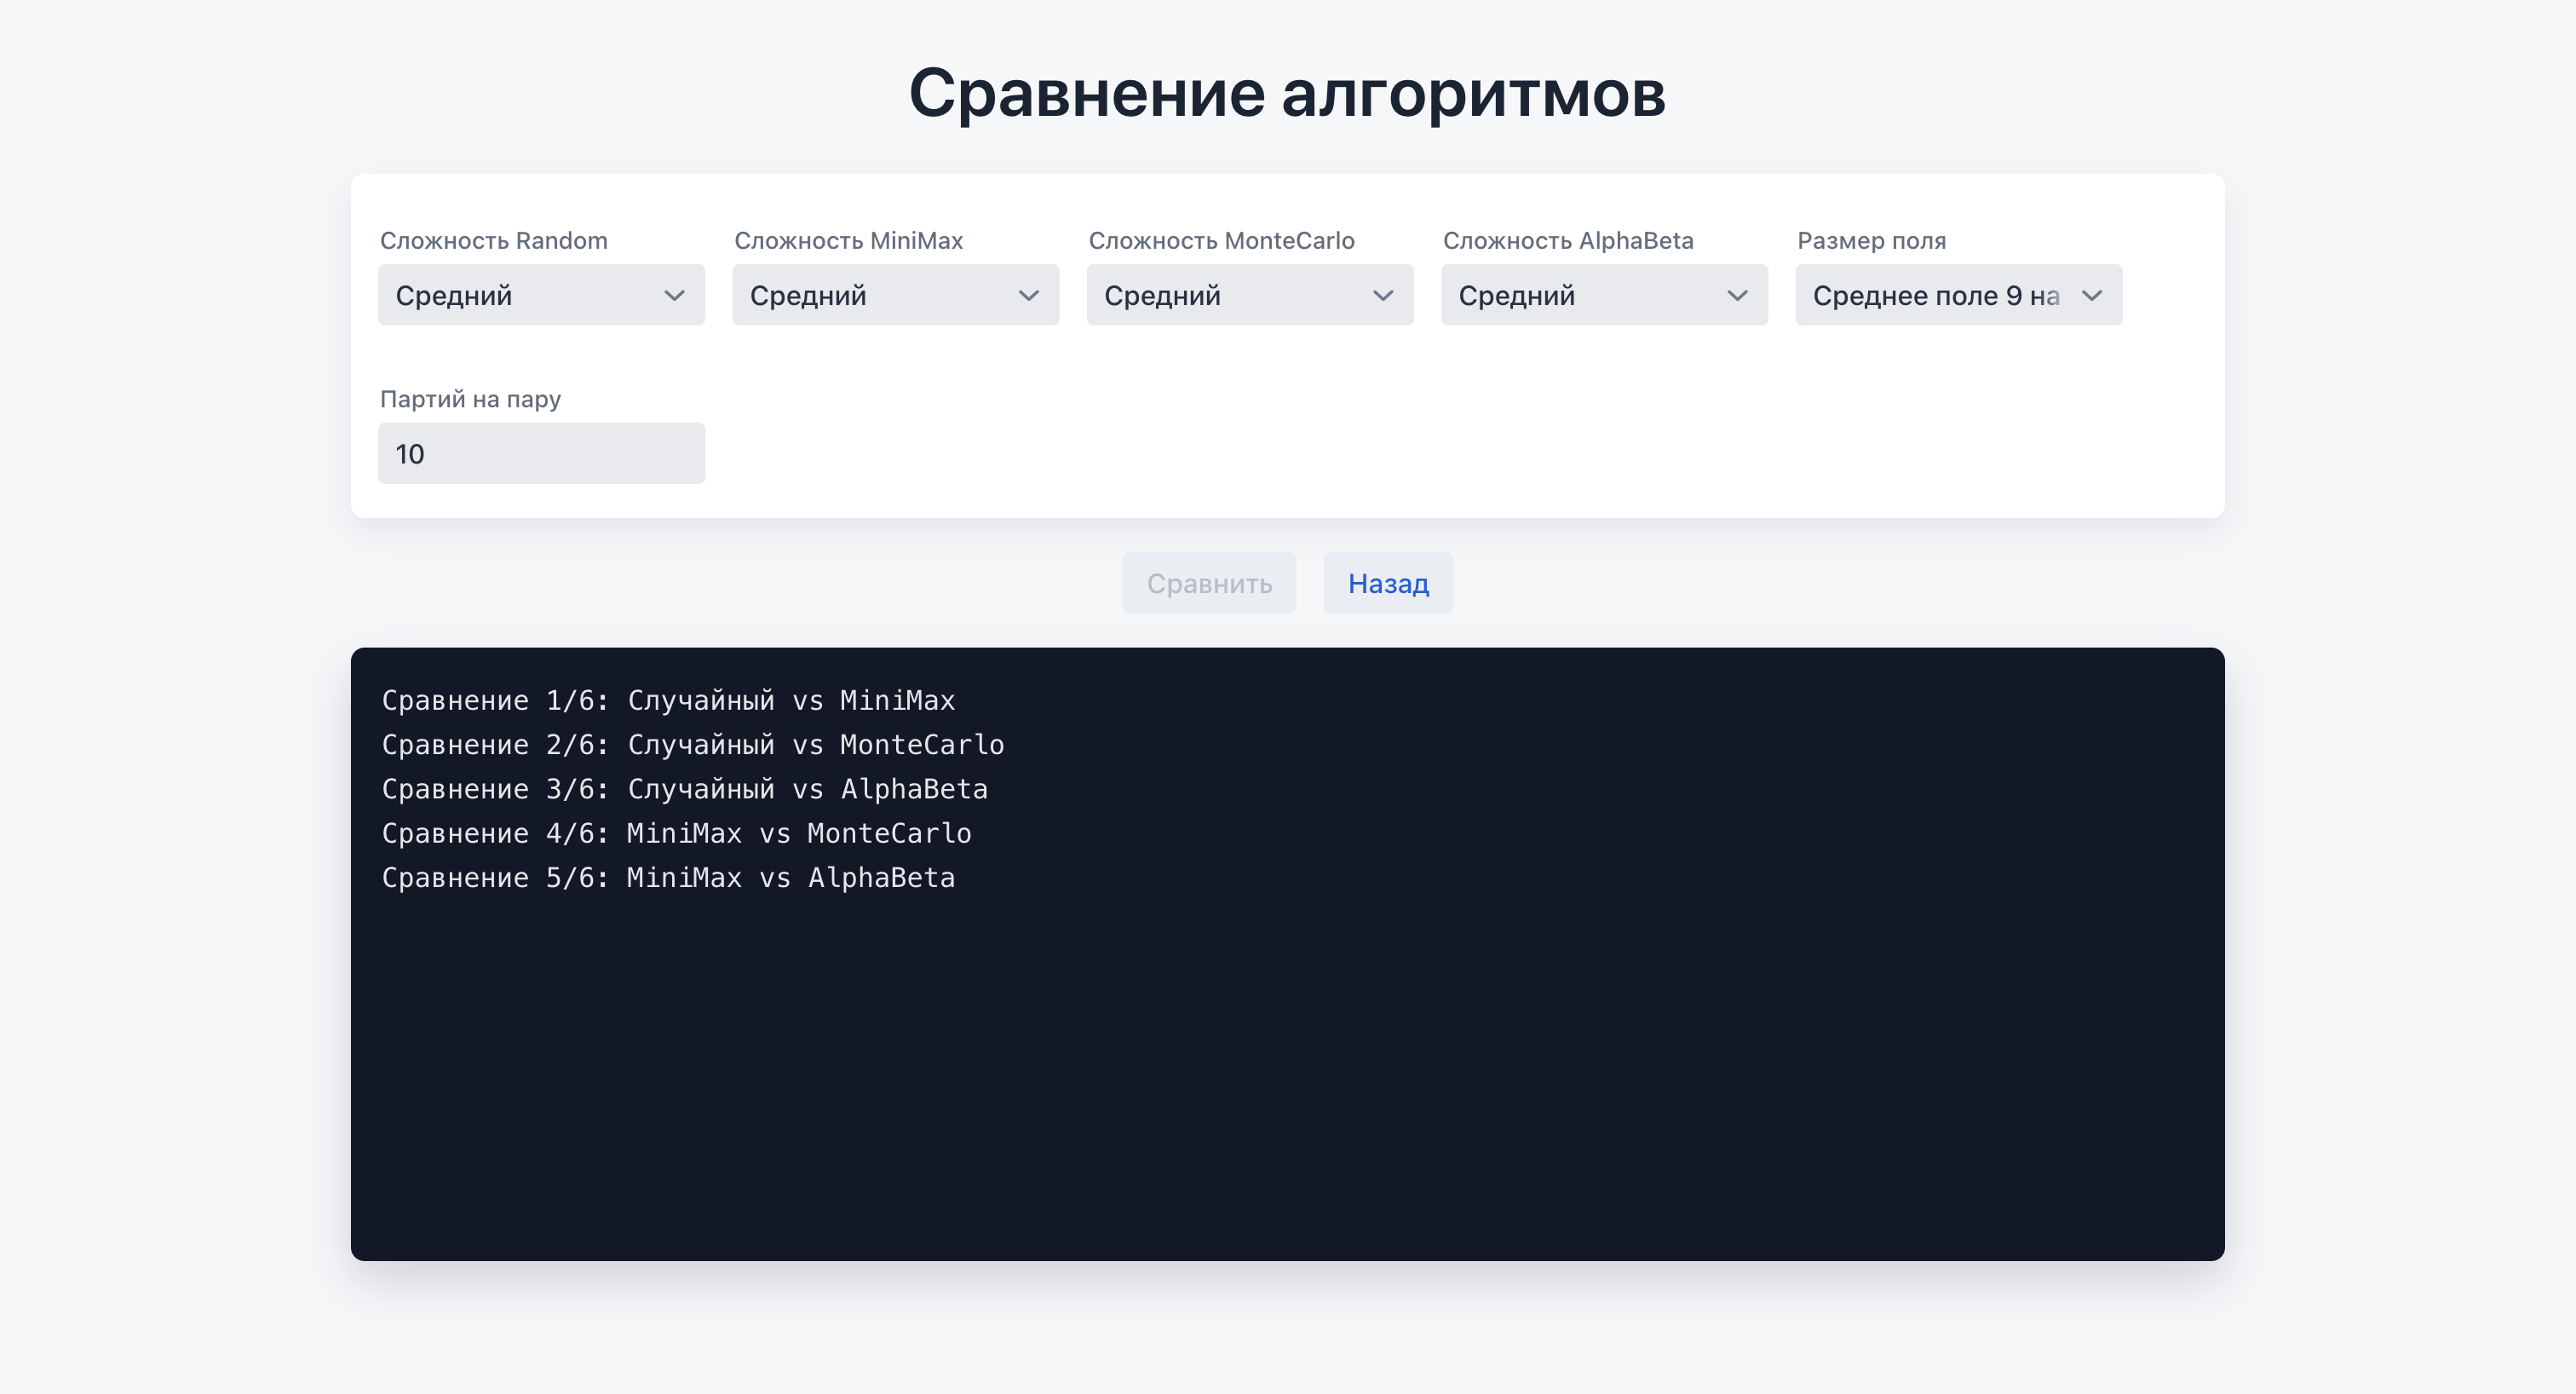
\includegraphics[width=0.88\textwidth]{comparison-page.png}
    \caption{Экран сравнения алгоритмов}
    \label{fig:comparison_page}
\end{figure}

\textit{Режим обучения весов} запускает серию self-play партий между двумя выбранными алгоритмами. По завершении каждой партии сервис обучения обновляет веса функции оценки, сохраняет их в файл и выводит ход эксперимента в лог. Пример логов обучения показан на рисунке~\ref{fig:training_page}.

\begin{figure}[h]
    \centering
    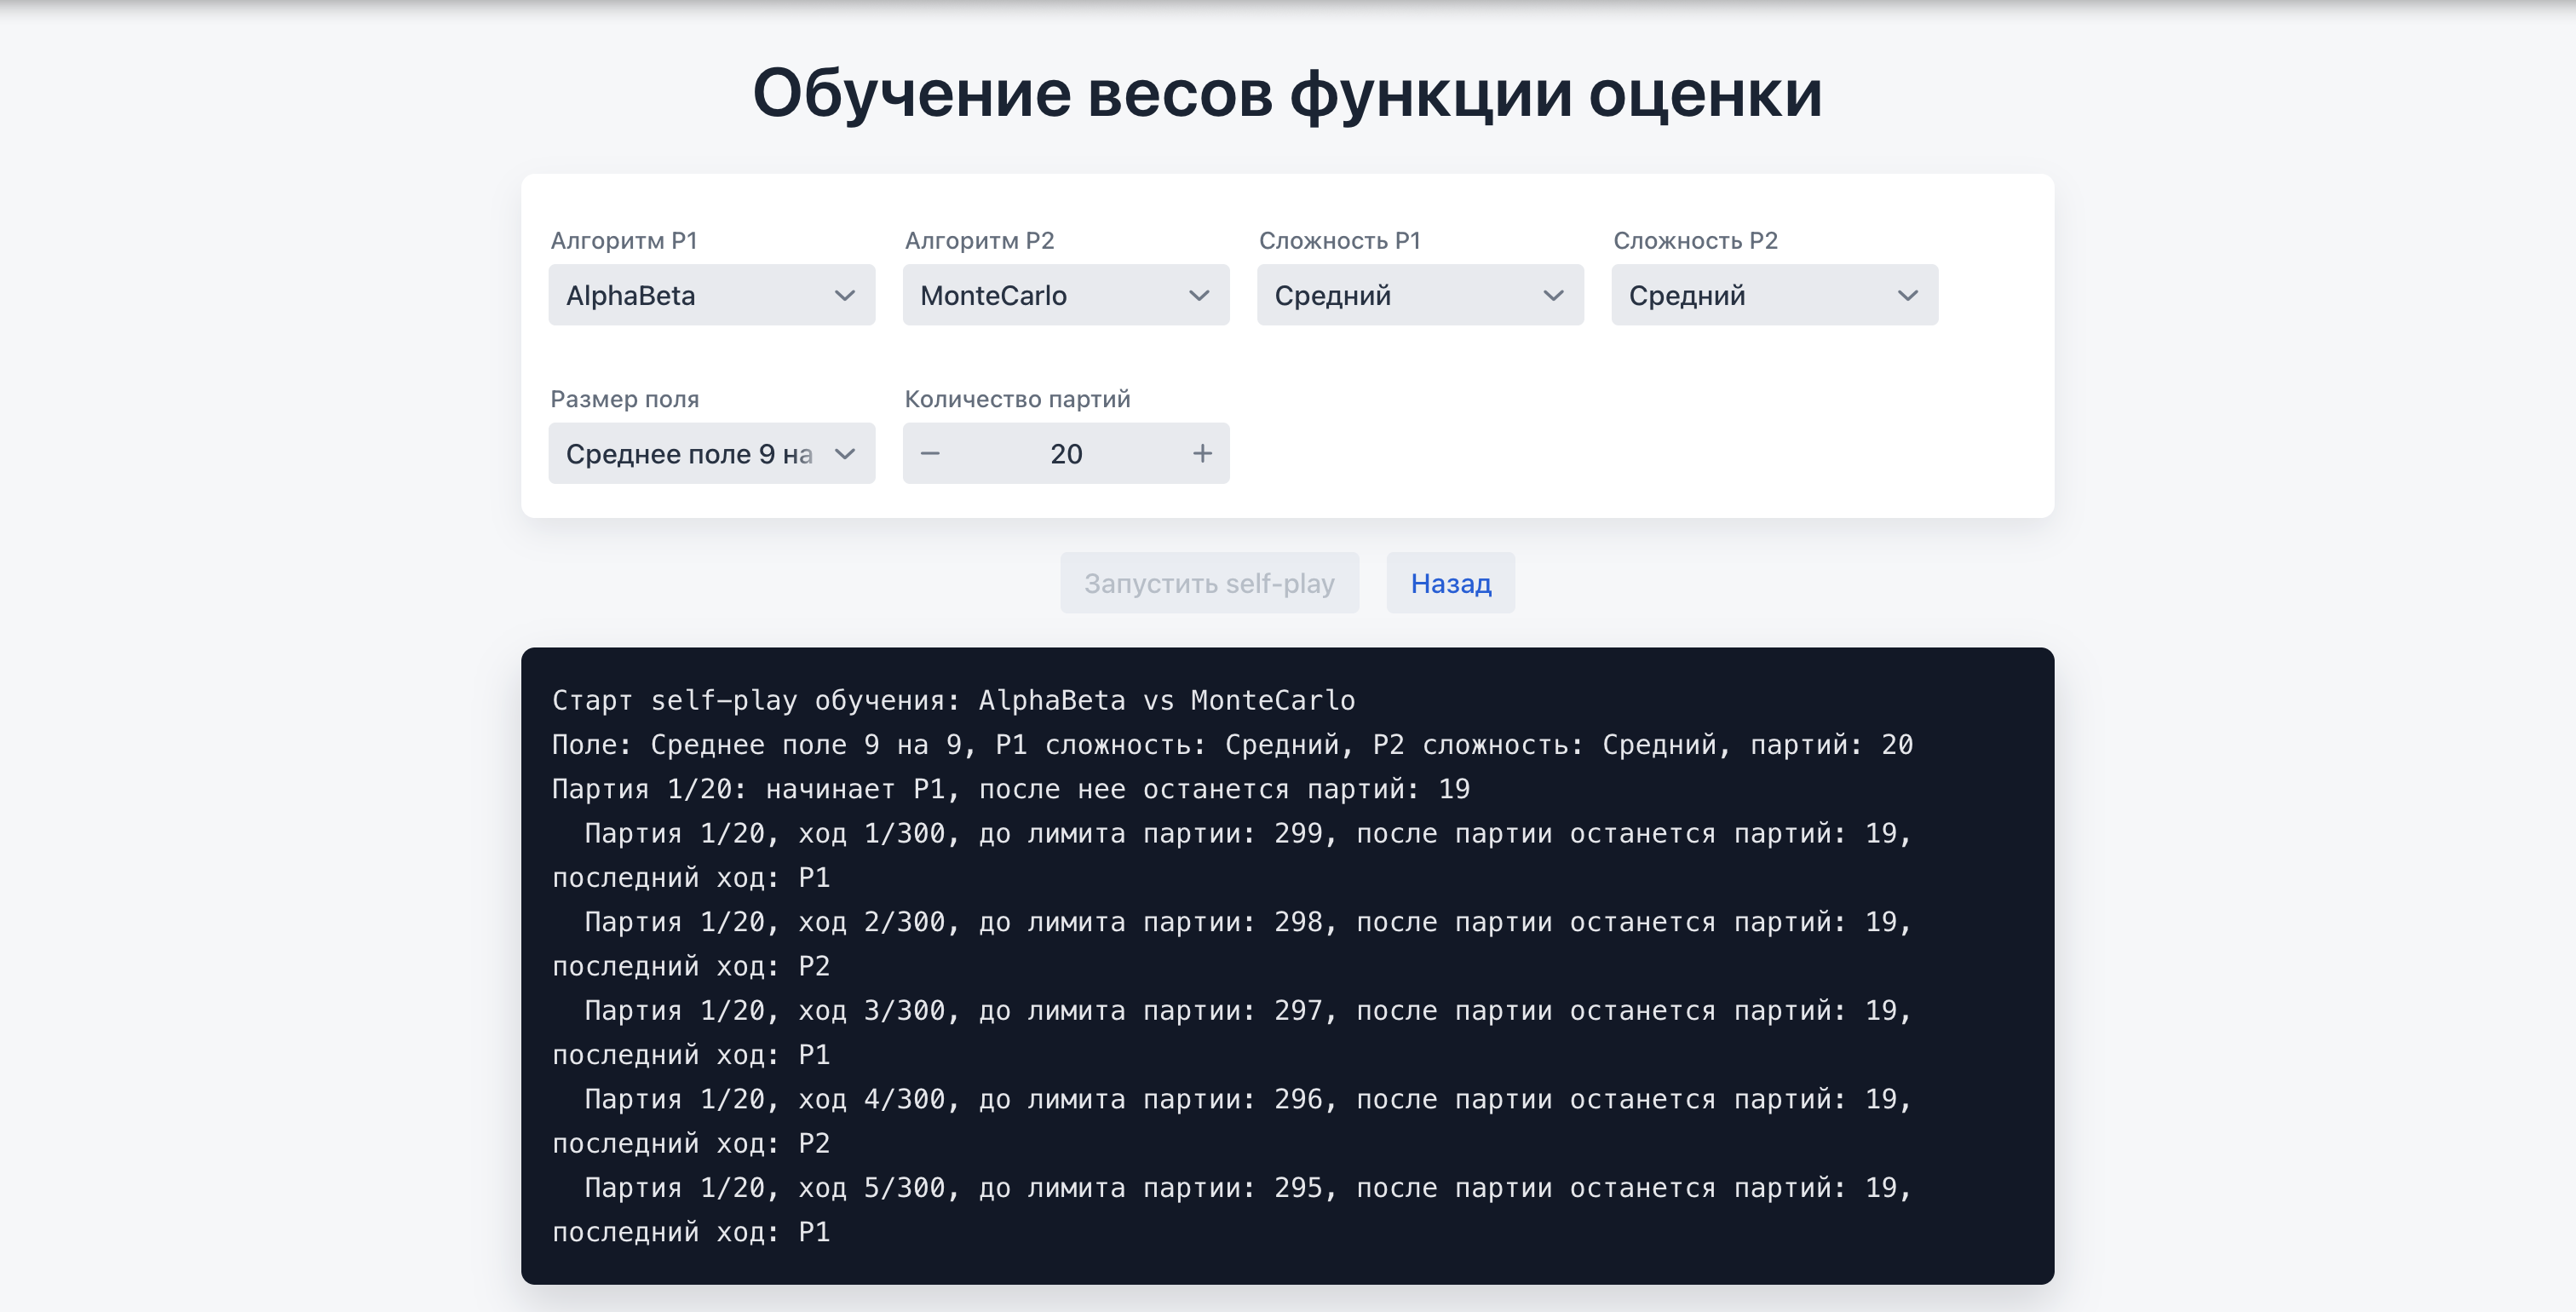
\includegraphics[width=0.88\textwidth]{training-page.png}
    \caption{Экран self-play обучения весов функции оценки}
    \label{fig:training_page}
\end{figure}

\chapter{Сравнение алгоритмов}

\section{Методика сравнения}

Сравнение алгоритмов выполняется в отдельном режиме приложения <<Сравнение алгоритмов>>. Цель режима "--- получить не единичный результат отдельной партии, а агрегированную оценку поведения стратегий на одинаковых условиях.

В эксперименте участвуют четыре алгоритма:
\begin{itemize}
    \item \texttt{RandomAlgorithm};
    \item \texttt{MinimaxAlgorithm};
    \item \texttt{AlphaBetaAlgorithm};
    \item \texttt{MonteCarloAlgorithm}.
\end{itemize}

Алгоритмы сравниваются попарно. Для исключения повторов рассматриваются только неупорядоченные пары: если матч \texttt{MiniMax} против \texttt{Random} уже проведён, обратная пара \texttt{Random} против \texttt{MiniMax} отдельно не запускается. При четырёх алгоритмах количество различных пар равно:

\[
    C_4^2 = \frac{4 \cdot 3}{2} = 6.
\]

Внутри каждой пары проводится заданное пользователем число партий. Для компенсации преимущества первого хода роли игроков чередуются: часть партий алгоритм проводит за первого игрока, часть "--- за второго. Размер поля и уровень сложности каждого алгоритма задаются перед запуском эксперимента.

Важно, что в режиме сравнения алгоритмов обучение весов функции оценки не выполняется. Это сделано намеренно: если во время эксперимента функция оценки будет изменяться, более поздние партии будут проходить уже при других условиях, и сравнение потеряет воспроизводимость. Поэтому веса считаются фиксированными на протяжении всего запуска сравнения.

\section{Собираемые метрики}

Для анализа недостаточно знать только победителя. Два алгоритма могут иметь близкую долю побед, но существенно отличаться по времени работы, глубине поиска или количеству просмотренных состояний. Поэтому приложение собирает несколько групп метрик.

\begin{table}[h]
    \centering
    \caption{Метрики сравнения алгоритмов}
    \label{tab:comparison_metrics}
    \begin{tabular}{lp{9cm}}
        \toprule
        Метрика & Смысл \\
        \midrule
        Количество партий & Общее число завершённых партий с участием алгоритма \\
        Победы, поражения, ничьи & Основная игровая результативность алгоритма \\
        Win rate & Доля побед алгоритма среди всех сыгранных им партий \\
        Среднее число ходов & Косвенная характеристика стиля игры и сложности партий \\
        Среднее время хода & Практическая вычислительная стоимость алгоритма \\
        Средняя глубина & Насколько глубоко алгоритм успевает просмотреть дерево \\
        Среднее число узлов & Объём реально просмотренного дерева поиска \\
        Среднее число отсечений & Эффективность alpha-beta оптимизации \\
        Попадания в TT & Эффективность таблицы транспозиций \\
        \bottomrule
    \end{tabular}
\end{table}

Метрики глубины, узлов, отсечений и попаданий в таблицу транспозиций особенно важны для сравнения \texttt{MiniMaxAlgorithm} и \texttt{AlphaBetaAlgorithm}. Оба алгоритма основаны на дереве игры, но альфа-бета должен просматривать меньше узлов при большей достижимой глубине. Для \texttt{MonteCarloAlgorithm} ключевыми являются число итераций и время хода, поскольку качество решения определяется количеством проведённых симуляций.

\section{План эксперимента}

Базовый эксперимент проводится на стандартном поле $9 \times 9$. Для каждого алгоритма устанавливается уровень сложности \texttt{MEDIUM}. Каждая пара алгоритмов играет по 10 партий. Тогда суммарное число партий равно:

\[
    6 \cdot 10 = 60.
\]

После базового эксперимента целесообразно провести дополнительный запуск на уровне \texttt{HARD}, поскольку именно на высоком уровне сложности сильнее проявляются различия между переборными алгоритмами. AlphaBeta получает возможность искать глубже за счёт отсечений, тогда как MiniMax ограничивается меньшей глубиной из-за экспоненциального роста дерева.

\section{Форма представления результатов}

Итоговая статистика может быть представлена в двух формах. Первая форма "--- попарная таблица побед, показывающая, как конкретные алгоритмы играют друг против друга.

\begin{table}[h]
    \centering
    \caption{Попарные результаты сравнения алгоритмов}
    \label{tab:tournament}
    \resizebox{\textwidth}{!}{%
    \begin{tabular}{llrrrrrrrrr}
        \toprule
        Алгоритм P1 & Алгоритм P2 & Игры & Победы P1 & Победы P2 & Ничьи & Ср. ходов & Ср. мс & Ср. глуб. & Ср. узлы & Ср. отсеч. / TT \\
        \midrule
        Случайный  & MiniMax    & 10 & 0 & 8  & 2 &  66{,}50 &  151{,}2 &  2{,}46 & 1088{,}5 &   0{,}0 /   0{,}0 \\
        Случайный  & MonteCarlo & 10 & 0 & 10 & 0 & 142{,}50 & 1051{,}7 & 31{,}67 &  140{,}8 &   0{,}0 /   0{,}0 \\
        Случайный  & AlphaBeta  & 10 & 0 & 10 & 0 &  73{,}50 &  412{,}4 &  3{,}41 & 1307{,}5 & 249{,}2 / 198{,}9 \\
        MiniMax    & MonteCarlo & 10 & 4 & 6  & 0 &  98{,}30 & 1360{,}1 & 33{,}00 &  947{,}1 &   0{,}0 /   0{,}0 \\
        MiniMax    & AlphaBeta  & 10 & 1 & 1  & 8 &  41{,}80 & 1215{,}3 &  4{,}85 & 4652{,}7 & 503{,}6 / 371{,}0 \\
        MonteCarlo & AlphaBeta  & 10 & 1 & 6  & 3 &  79{,}90 & 1839{,}7 & 34{,}28 & 1504{,}6 & 266{,}5 / 217{,}4 \\
        \bottomrule
    \end{tabular}%
    }
\end{table}

Вторая форма "--- агрегированная таблица по каждому алгоритму. Она удобнее для общего вывода, поскольку показывает не только победы, но и вычислительные затраты.

\begin{table}[h]
    \centering
    \caption{Сводная статистика алгоритмов}
    \label{tab:summary_metrics}
    \resizebox{\textwidth}{!}{%
    \begin{tabular}{lrrrrrrrrrrr}
        \toprule
        Алгоритм & Партий & Победы & Поражения & Ничьи & Winrate & Очки/партия & Ср. ходов & Ср. мс & Ср. глуб. & Ср. узлы & Ср. отсеч. / TT \\
        \midrule
        Случайный  & 30 &  0 & 28 &  2 &  0{,}00\% & 0{,}03 &  94{,}17 &  538{,}4 & 12{,}51 &  845{,}6 &  83{,}1 /  66{,}3 \\
        MiniMax    & 30 & 13 &  7 & 10 & 43{,}33\% & 0{,}60 &  68{,}87 &  908{,}9 & 13{,}44 & 2229{,}4 & 167{,}9 / 123{,}7 \\
        MonteCarlo & 30 & 17 & 10 &  3 & 56{,}67\% & 0{,}62 & 106{,}90 & 1417{,}2 & 32{,}98 &  864{,}2 &  88{,}8 /  72{,}5 \\
        AlphaBeta  & 30 & 17 &  2 & 11 & 56{,}67\% & 0{,}75 &  65{,}07 & 1155{,}8 & 14{,}18 & 2488{,}3 & 339{,}8 / 262{,}4 \\
        \bottomrule
    \end{tabular}%
    }
\end{table}

Для AlphaBeta дополнительно анализируются среднее число отсечений и попаданий в таблицу транспозиций. Эти показатели позволяют подтвердить, что улучшение относительно MiniMax связано не только с увеличенным лимитом времени, но и с реальным сокращением числа просматриваемых ветвей.

\section{Анализ результатов}

Фактические результаты подтверждают, что случайный алгоритм является базовой линией: за 30 партий он не одержал ни одной победы и набрал только две ничьи. Это ожидаемо, поскольку даже при использовании функции оценки он не строит дерево последствий и не анализирует ответы соперника.

MiniMax заметно сильнее случайного алгоритма: он выиграл 13 партий из 30 и набрал 0{,}60 очка за партию. При этом его слабое место сохраняется "--- экспоненциальный рост числа состояний. Даже при ограничении ширины до 16 ходов глубина 5 даёт до $16^5 \approx 1{,}05 \cdot 10^6$ узлов в худшем случае, поэтому алгоритм вынужден жёстко ограничивать глубину и ширину перебора.

AlphaBeta показал лучший интегральный результат: 17 побед, только 2 поражения и 0{,}75 очка за партию. При равном winrate с MonteCarlo он имеет меньше поражений и больше ничьих, что говорит о более устойчивом поведении в сложных позициях. Среднее число отсечений 339{,}8 и 262{,}4 попадания в таблицу транспозиций за ход подтверждают, что преимущество алгоритма связано не только с перебором, но и с эффективным сокращением дерева поиска.

MonteCarlo также показал высокий результат "--- 17 побед из 30 и winrate 56{,}67\%. Его партии в среднем длиннее, чем у AlphaBeta, а среднее время хода выше. Это отражает природу метода: качество решения зависит от числа симуляций и устойчивости rollout-стратегии. В игре <<Коридор>> это особенно важно из-за большого числа возможных стен: если бюджет итераций мал, статистика по отдельным ходам может быть недостаточно устойчивой.

\section{Ограничения эксперимента}

При интерпретации результатов необходимо учитывать несколько ограничений.

Во-первых, алгоритмы используют разные типы вычислительного бюджета: MiniMax и AlphaBeta ограничены глубиной и временем, а MCTS "--- временем, числом итераций и глубиной симуляции. Поэтому сравнение не является сравнением <<одинаковых>> алгоритмов при одинаковой глубине, а является сравнением реализованных игровых стратегий в условиях приложения.

Во-вторых, результат зависит от текущих весов функции оценки. Для воспроизводимости в тексте работы необходимо указать значения весов из файла \texttt{data/evaluation-weights.properties}, использованные перед запуском эксперимента.

В-третьих, выбор числа партий влияет на статистическую устойчивость результатов. Серия из 60 партий подходит для первичного сравнения, но для более надёжного вывода желательно увеличить число партий в каждой паре.

\chapternonum{Заключение}

В ходе выполнения выпускной квалификационной работы была исследована настольная логическая игра <<Коридор>> и построена её графовая модель. Реализованы алгоритмы проверки корректности перемещения фишки с учётом всех правил прыжков через соперника и проверки корректности установки перегородки через обход графа в ширину. Реализован алгоритм поиска кратчайшего пути до целевой линии на основе BFS с восстановлением пути.

Разработана многофакторная функция оценки позиции, учитывающая семь признаков: разность длин путей, мобильность фишек, преимущество в перегородках, продвижение к цели и эндшпильные бонусы. Реализован механизм коррекции весов функции оценки по результатам завершённых партий с сохранением в файл конфигурации между сессиями.

Реализованы четыре алгоритма программного соперника с тремя уровнями сложности каждый. Случайный алгоритм служит базовой линией. Минимакс с кэшированием и ограничением ширины перебора обеспечивает разумный баланс качества и скорости. Минимакс с альфа-бета отсечением, сортировкой ходов, таблицей транспозиций с типами границ и затухающим поиском в шумных позициях является наиболее сильным из переборных алгоритмов. Метод Монте-Карло с UCT, эвристическим выбором ходов в симуляциях и условием досрочного останова обеспечивает альтернативный подход, основанный на статистике симуляций.

Разработано игровое приложение с режимами <<Игрок против ИИ>>, <<ИИ против ИИ>>, режимом подсказок одновременно от всех четырёх алгоритмов, режимом воспроизведения партии, турнирным режимом и режимом сравнения алгоритмов. После проведения экспериментального запуска таблицы сравнения алгоритмов должны быть заполнены фактическими результатами.

\renewcommand\bibname{Список литературы}
\bibliographystyle{ugost2003}
\bibliography{quoridorBibliography}

\appendix

\lstset{
    language=Java,
    breaklines=true,
    tabsize=4,
    formfeed=\newpage,
    extendedchars=true,
    texcl=true,
    basicstyle=\ttfamily,
    commentstyle=\rmfamily\itshape,
    stringstyle=\slshape,
    numbers=left,
    numbersep=1em,
    stepnumber=1,
    numberstyle=\footnotesize\color{black},
    literate=
        {а}{{\cyra}}1 {б}{{\cyrb}}1 {в}{{\cyrv}}1 {г}{{\cyrg}}1 {д}{{\cyrd}}1
        {е}{{\cyre}}1 {ё}{{\cyryo}}1 {ж}{{\cyrzh}}1 {з}{{\cyrz}}1 {и}{{\cyri}}1
        {й}{{\cyrishrt}}1 {к}{{\cyrk}}1 {л}{{\cyrl}}1 {м}{{\cyrm}}1 {н}{{\cyrn}}1
        {о}{{\cyro}}1 {п}{{\cyrp}}1 {р}{{\cyrr}}1 {с}{{\cyrs}}1 {т}{{\cyrt}}1
        {у}{{\cyru}}1 {ф}{{\cyrf}}1 {х}{{\cyrh}}1 {ц}{{\cyrc}}1 {ч}{{\cyrch}}1
        {ш}{{\cyrsh}}1 {щ}{{\cyrshch}}1 {ъ}{{\cyrhrdsn}}1 {ы}{{\cyrery}}1
        {ь}{{\cyrsftsn}}1 {э}{{\cyrerev}}1 {ю}{{\cyryu}}1 {я}{{\cyrya}}1
        {А}{{\CYRA}}1 {Б}{{\CYRB}}1 {В}{{\CYRV}}1 {Г}{{\CYRG}}1 {Д}{{\CYRD}}1
        {Е}{{\CYRE}}1 {Ё}{{\CYRYO}}1 {Ж}{{\CYRZH}}1 {З}{{\CYRZ}}1 {И}{{\CYRI}}1
        {Й}{{\CYRISHRT}}1 {К}{{\CYRK}}1 {Л}{{\CYRL}}1 {М}{{\CYRM}}1 {Н}{{\CYRN}}1
        {О}{{\CYRO}}1 {П}{{\CYRP}}1 {Р}{{\CYRR}}1 {С}{{\CYRS}}1 {Т}{{\CYRT}}1
        {У}{{\CYRU}}1 {Ф}{{\CYRF}}1 {Х}{{\CYRH}}1 {Ц}{{\CYRC}}1 {Ч}{{\CYRCH}}1
        {Ш}{{\CYRSH}}1 {Щ}{{\CYRSHCH}}1 {Ъ}{{\CYRHRDSN}}1 {Ы}{{\CYRERY}}1
        {Ь}{{\CYRSFTSN}}1 {Э}{{\CYREREV}}1 {Ю}{{\CYRYU}}1 {Я}{{\CYRYA}}1
        {—}{{---}}1 {–}{{--}}1 {«}{{<<}}1 {»}{{>>}}1
}

\chapter{Реализация интерфейса алгоритма}

\lstinputlisting[
    caption={Интерфейс \texttt{Algorithm}},
    label={lst:algorithm_interface},
    firstline=13
]{../src/main/java/ru/ac/uniyar/model/algorithms/Algorithm.java}

\chapter{Реализация случайного алгоритма}

\lstinputlisting[
    caption={Класс \texttt{RandomAlgorithm}},
    label={lst:random_algorithm},
    firstline=12
]{../src/main/java/ru/ac/uniyar/model/algorithms/RandomAlgorithm.java}

\chapter{Реализация алгоритма MiniMax}

\lstinputlisting[
    caption={Класс \texttt{MinimaxAlgorithm}},
    label={lst:minimax_algorithm},
    firstline=10
]{../src/main/java/ru/ac/uniyar/model/algorithms/MinimaxAlgorithm.java}

\chapter{Реализация алгоритма AlphaBeta}

\lstinputlisting[
    caption={Класс \texttt{AlphaBetaAlgorithm}},
    label={lst:alphabeta_algorithm},
    firstline=8
]{../src/main/java/ru/ac/uniyar/model/algorithms/AlphaBetaAlgorithm.java}

\chapter{Реализация алгоритма Monte Carlo}

\lstinputlisting[
    caption={Класс \texttt{MonteCarloAlgorithm}},
    label={lst:mcts_algorithm},
    firstline=10
]{../src/main/java/ru/ac/uniyar/model/algorithms/MonteCarloAlgorithm.java}

\chapter{Реализация обучения весов функции оценки}

\lstinputlisting[
    caption={Класс \texttt{EvaluationWeightsStore}},
    label={lst:evaluation_weights_store},
    firstline=13
]{../src/main/java/ru/ac/uniyar/model/algorithms/EvaluationWeightsStore.java}

\end{document}
